\section{Моделирование волновых процессов в многослойных средах}

\todo{Перенести сюда материалы про многослойки}

\clearpage
\newpage

\section{Моделирование низкоскоростного удара по композитной конструкции}

В данном разделе приведены результаты численного моделирования низкоскоростного
удара по композитной конструкции.

Рассматривается задача о динамическом нагружении элемента композитной обшивки крыла самолёта. На рис.
\ref{pic:construction} приведена схема строения обшивки и силового кессона
крыла, выполненных из композиционных материалов. Обшивка толщиной 6.5~мм состоит 
из 3 композитных субпакетов, стрингер толщиной 13~мм -- из 6 аналогичных субпакетов. Каждый субпакет
состоит из 11 монослоёв со взаимной ориентацией субпакетов при укладке 
45/0/-45/0/0/90/0/0/-45/0/45. Каждый монослой имеет следующий состав: 60\% -- 
ориентированные длинные углепластиковые волокна; 40\% -- матрица
(эпоксидная смола). 

\begin{figure}[h]
\center{\includegraphics[width=\textwidth]{png/construction.png}}
\caption{Обшивка и силовой кессон крыла.}
\label{pic:construction}
\end{figure}

Низкоскоростной удар (от метров в секунду до десятков метров в секунду) 
как правило не приводит к пробиванию и разрушению композитной панели. Однако, 
характеристики конструкции значительно ухудшаются, вплоть до полной непригодности к 
дальнейшей эксплуатации. Это связано с внутренними повреждениями и разрушениями 
в композитном материале. Так, многослойные материалы после нагрузок могут заметно 
терять прочность даже при отсутствии видимых поврежедний.
Это обусловлено появлением внутренних микротрещин, которые впоследствии, объединяясь,
превращаются в макротрещины. Возникающие после нагрузки повреждения
материала могут быть визуально не заметны, хотя делают образец непригодным к
дальнейшему использованию.

Сложное внутреннее строение и многоуровневость структуры композитных материалов вносят несколько 
принципиальных факторов, влияющих на их прочностные свойства.

\begin{itemize}

\item Динамическое воздействие по конструкции вызывает в ней распространение упругих и пластических волн 
нагрузки. В случае композитного материала множественные переотражения волн от внутренних контактных 
границ формируют сложную волновую картину. Интерференция большого количества 
прямых, отражённых и преломлённых волн определяет итоговые области максимальных нагрузок в конструкции. 
Таким образом, внутреннее строение композита влияет на то, где будут локализованы области 
повреждений различных видов.

\item Наличие микроструктуры композита (уровень отдельных волокон в матрице) приводит к появлению зон 
концентрации напряжений. В результате могут заметно снижаться предельные значения напряжений, которые 
выдерживают матрица и волокна в составе композитной конструкции, по сравнению с аналогичными значениями
для изотропных образцов из тех же материалов.

\end{itemize}

В связи с приведёнными фактами одной из актуальных прикладных задач, связанных с прочностными испытаниями 
композитных материалов, является задача о получении волновой картины в образце после
непробивающего удара. 

В эксперименте по непробивающему воздействию на обшивку нагрузка создается 
стальным ударником диаметром 25.4~мм. Характерный пример профиля нагрузки 
при испытаниях приведен на рис. \ref{pic:loadprofile}.
\begin{figure}[h]
\center{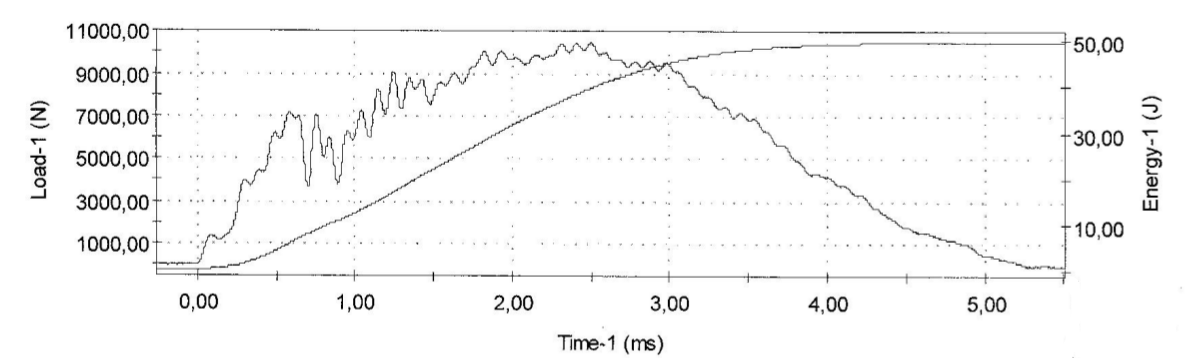
\includegraphics[width=\textwidth]{png/load-profile.png}}
\caption{Пример профиля нагрузки на обшивку крыла при испытаниях.}
\label{pic:loadprofile}
\end{figure}

Ввиду большой вычислительной сложности при моделировании подобной конструкции с 
точностью до отдельного волокна, а также из-за многообразия протекающих процессов, 
полная задача декомпозируется на ряд подзадач. В данном разделе рассматривается задача о получении
волновой картины в элементе композитной обшивки крыла в следующем приближении:
\begin{itemize}
\item конструкция состоит из композитных субпакетов, сооединённых эпоксидной смолой;
\item структура задаётся до уровня отдельного субпакета, монослои в расчёте не выделяются.
\end{itemize}

В данном приближении характеристики субпакетов принимаются равными характеристикам монослоёв, из которых они составлены. 
Анизотропия ниже уровня субпакета, обусловленная укладкой монослоёв внутри субпакета, не рассматривается. Характеристики материалов приведены в табл. \ref{tbl:subpackage} и \ref{tbl:max_stresses}.

\begin{table}
\centering
\begin{tabular}{|c|c|c|c|c|c|c|c|}
\hline
Материал & E, ГПа & $\nu$ & $\rho$, кг/м$^{3}$ & $\lambda$, ГПа & $\mu$, ГПа &
$c_p$, м/с & $c_s$, м/с \\
\hline
Монослой (субпакет) & 8.5 & 0.32 & 1580 & 5.72 & 3.22 & 2775 & 1425 \\
Эпоксидная смола & 2.5 & 0.30 & 1250 & 1.44 & 0.96 & 1640 & 876 \\
Сталь & 200 & 0.28 & 7800 & 99.43 & 78.13 & 5725 & 3165 \\
\hline
\end{tabular}
\caption{Упругие характеристики слоёв и ударника.}
\label{tbl:subpackage}
\end{table}

\begin{table}
\centering
\begin{tabular}{|c|c|}
\hline
Тип нагрузки & Предельно допустимая нагрузка, МПа \\
\hline
Растяжение вдоль волокон & 2630 \\
Сжатие вдоль волокон & 1530 \\
Растяжение поперёк волокон & 86 \\
Сжатие поперёк волокон & 213 \\
Сдвиг & 112 \\
\hline
\end{tabular}
\caption{Прочностные характеристики монослоёв.}
\label{tbl:max_stresses}
\end{table}


Были проведены расчеты для двух постановок эксперимента - удар по отдельному элементу обшивки и удар по элементу обшивки со стрингером. Вид расчетных областей приведен на рис. \ref{pic:wing_only_scene} и \ref{pic:wing_stringer_scene} соответственно. Часть расчётной сетки показана на рис. \ref{pic:wing_mesh_sample}. Скорость ударника в обоих расчётах составляет 6 м/с.

\begin{figure}[htp]
\center{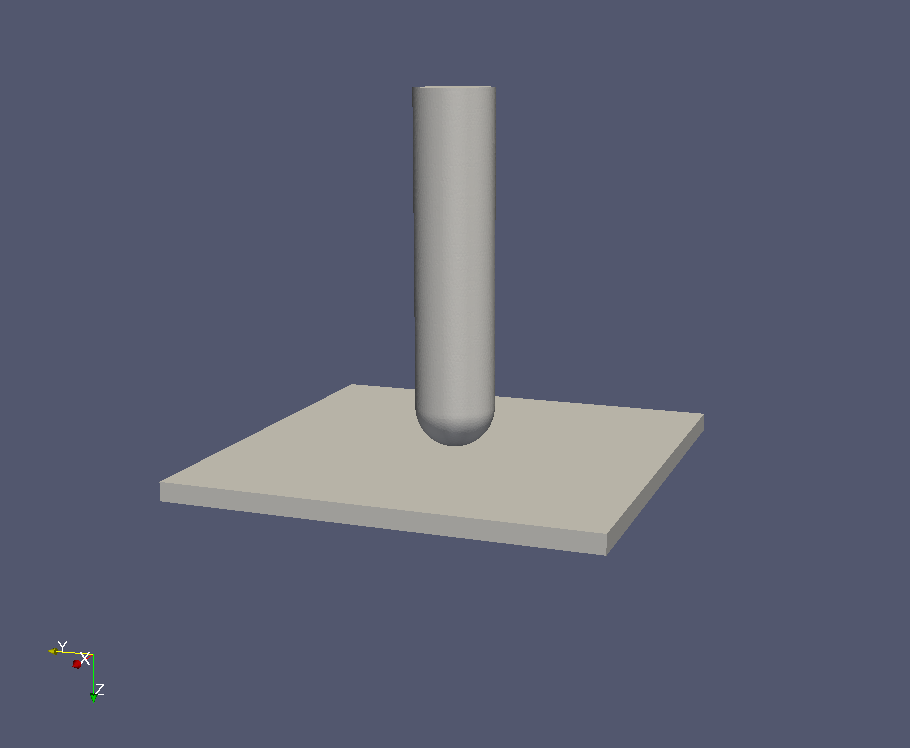
\includegraphics[width=0.75\textwidth]{png/pkm-experiment/wing-only/scene.png}}
\caption{Удар по элементу обшивки. Вид расчетной области.}
\label{pic:wing_only_scene}
\end{figure}

\begin{figure}[htp]
\center{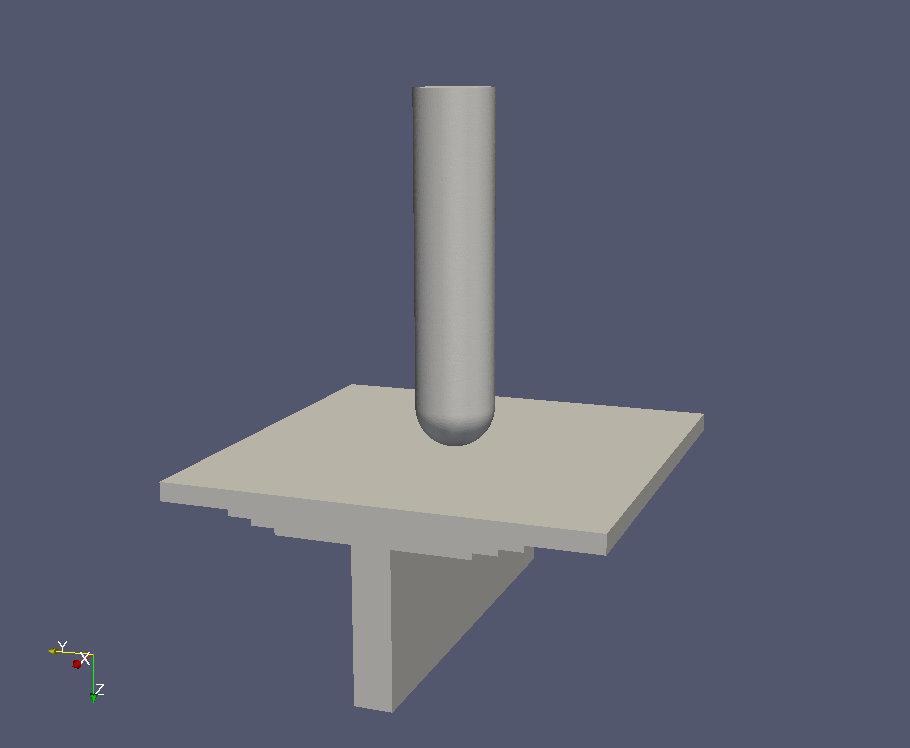
\includegraphics[width=0.75\textwidth]{png/pkm-experiment/wing-stringer/scene.png}}
\caption{Удар по элементу обшивки со стрингером. Вид расчетной области.}
\label{pic:wing_stringer_scene}
\end{figure}

\begin{figure}[htp]
\center{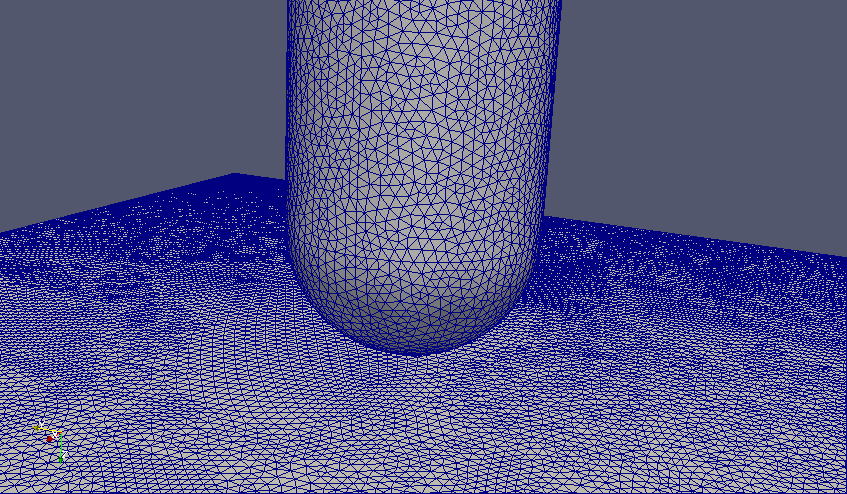
\includegraphics[width=0.75\textwidth]{png/pkm-experiment/mesh.png}}
\caption{Расчётная сетка. Поверхностная сетка в элементе крыла и в ударнике в районе места удара.}
\label{pic:wing_mesh_sample}
\end{figure}


На рис. \ref{pic:pkm_experiment_v3d_wing_only} показана общая форма трёхмерного возмущения в конструкции для постановки с отдельным элементом обшивки, а на рис. \ref{pic:pkm_experiment_v3d_wing_stringer} -- для постановки с элементом обшивки и стрингером.

\begin{figure}[htp]
\begin{subfigure}[b]{0.5\textwidth}
\centering
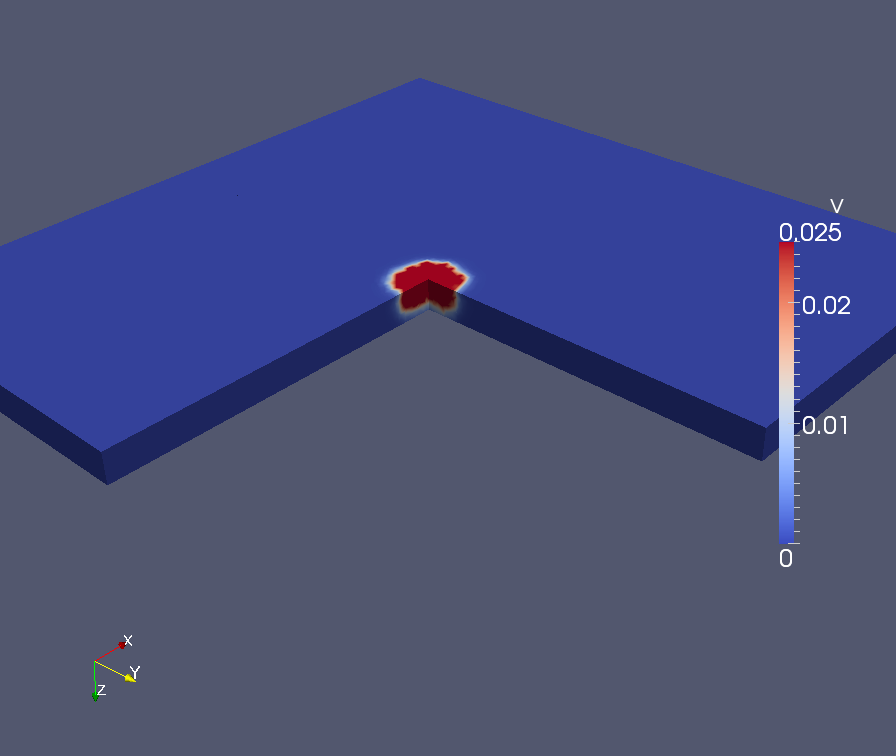
\includegraphics[width=\textwidth]{png/pkm-experiment/wing-only/wave-3d/v-0001.png}
\caption{0.5 мкс}
\end{subfigure}
\begin{subfigure}[b]{0.5\textwidth}
\centering
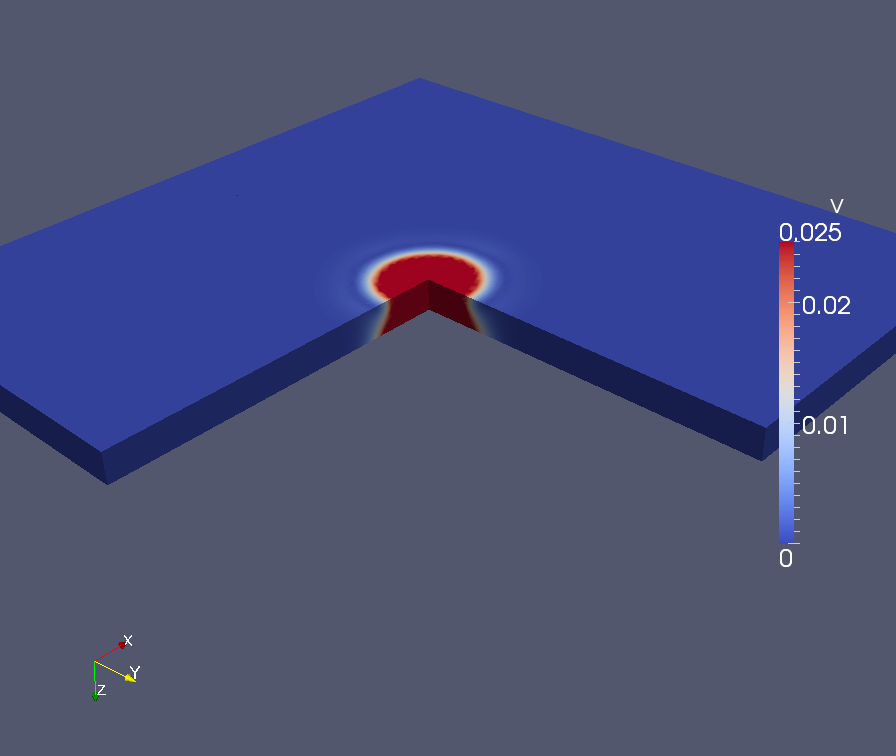
\includegraphics[width=\textwidth]{png/pkm-experiment/wing-only/wave-3d/v-0005.png}
\caption{3.0 мкс}
\end{subfigure}
\begin{subfigure}[b]{0.5\textwidth}
\centering
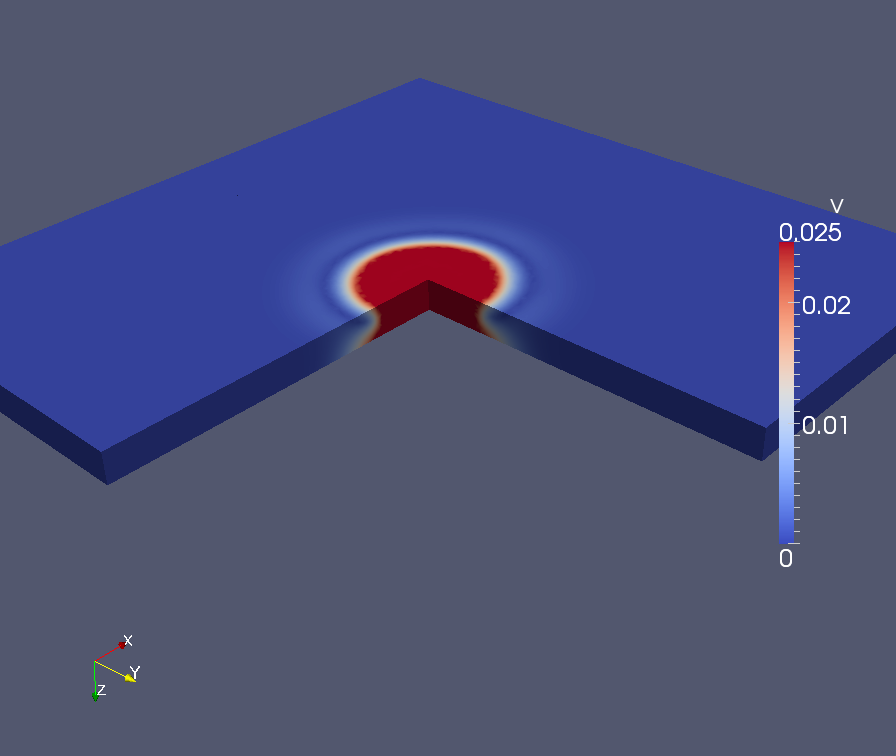
\includegraphics[width=\textwidth]{png/pkm-experiment/wing-only/wave-3d/v-0009.png}
\caption{5.5 мкс}
\end{subfigure}
\begin{subfigure}[b]{0.5\textwidth}
\centering
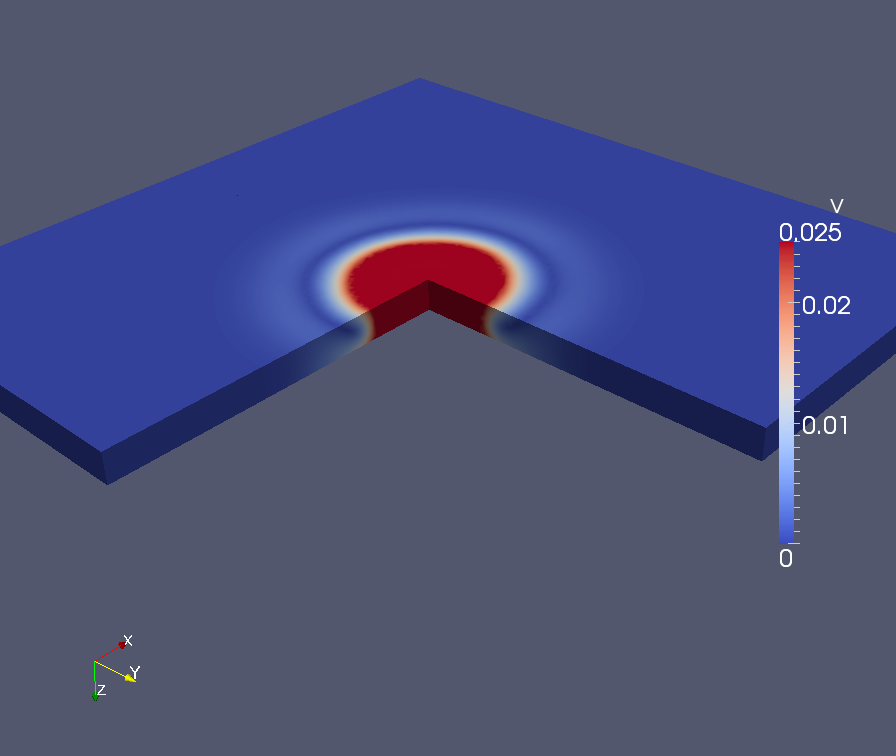
\includegraphics[width=\textwidth]{png/pkm-experiment/wing-only/wave-3d/v-0013.png}
\caption{8.0 мкс}
\end{subfigure}
\begin{subfigure}[b]{0.5\textwidth}
\centering
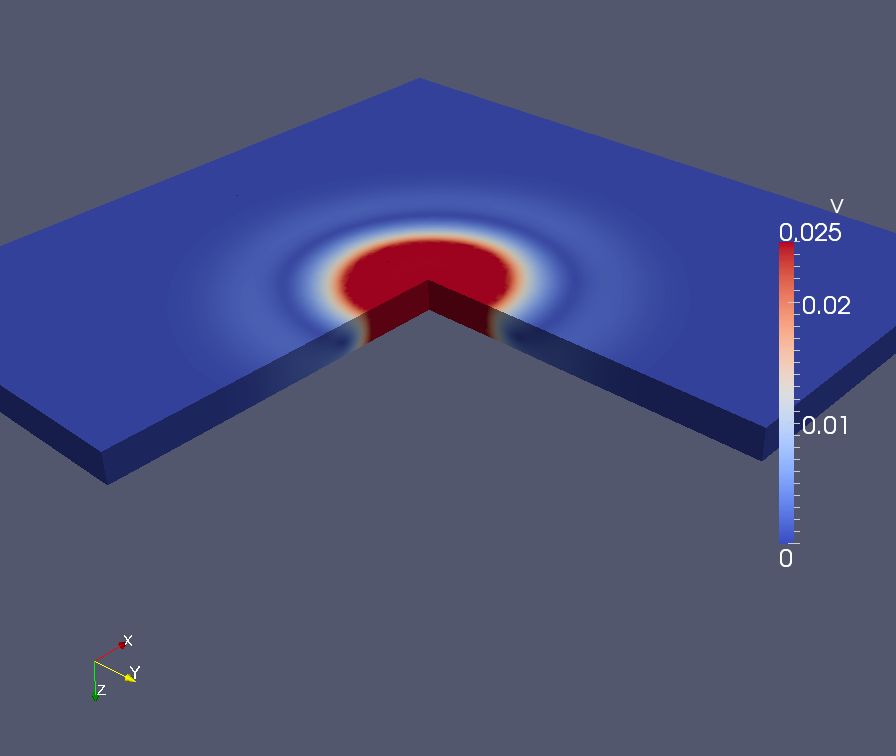
\includegraphics[width=\textwidth]{png/pkm-experiment/wing-only/wave-3d/v-0017.png}
\caption{10.5 мкс}
\end{subfigure}
\begin{subfigure}[b]{0.5\textwidth}
\centering
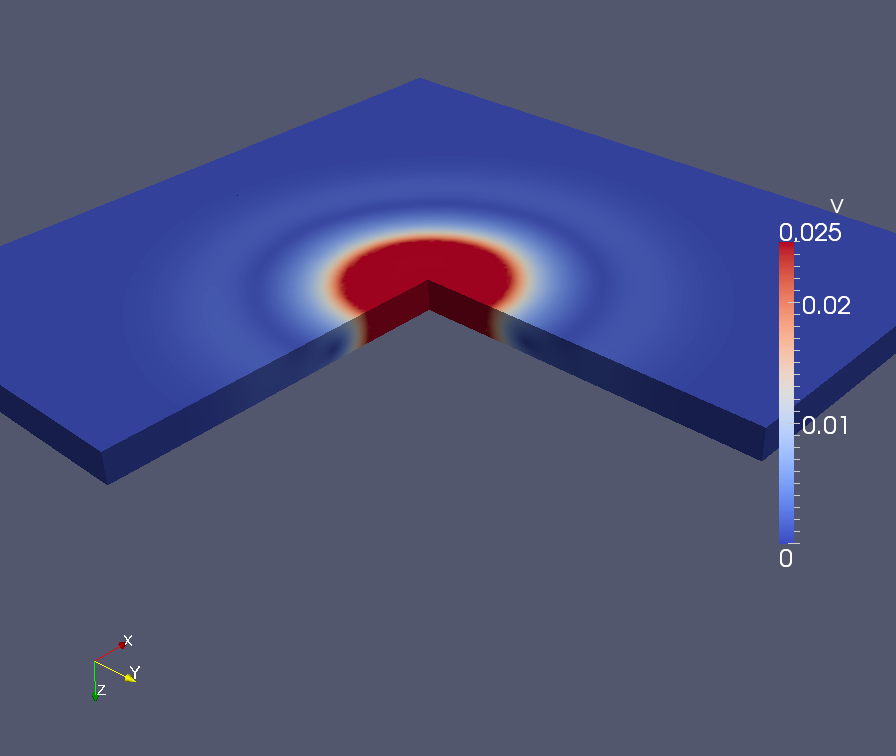
\includegraphics[width=\textwidth]{png/pkm-experiment/wing-only/wave-3d/v-0021.png}
\caption{13.0 мкс}
\end{subfigure}
\caption{Распространение возмущений в элементе обшивки. Общая картина. Цветом показан модуль скорости.}
\label{pic:pkm_experiment_v3d_wing_only}
\end{figure}


\begin{figure}[htp]
\begin{subfigure}[b]{0.5\textwidth}
\centering
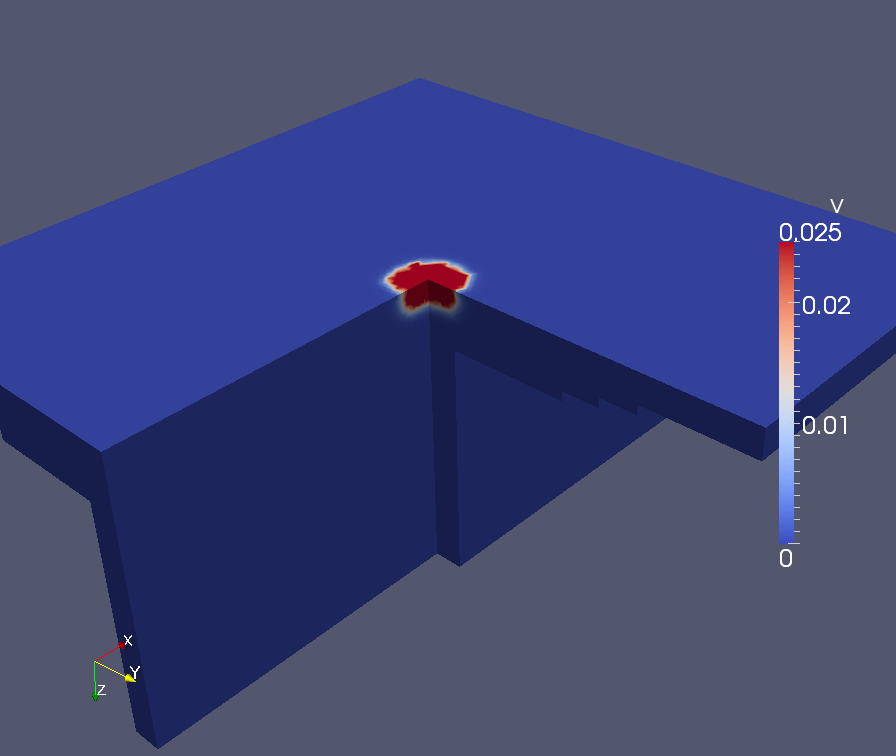
\includegraphics[width=\textwidth]{png/pkm-experiment/wing-stringer/wave-3d/v-0001.png}
\caption{0.5 мкс}
\end{subfigure}
\begin{subfigure}[b]{0.5\textwidth}
\centering
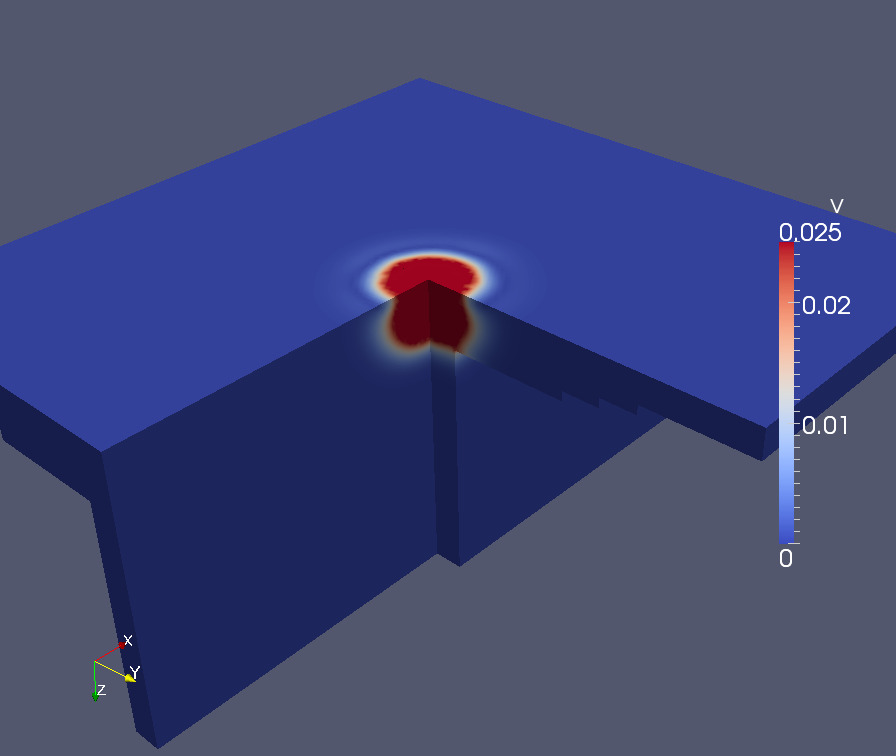
\includegraphics[width=\textwidth]{png/pkm-experiment/wing-stringer/wave-3d/v-0005.png}
\caption{3.0 мкс}
\end{subfigure}
\begin{subfigure}[b]{0.5\textwidth}
\centering
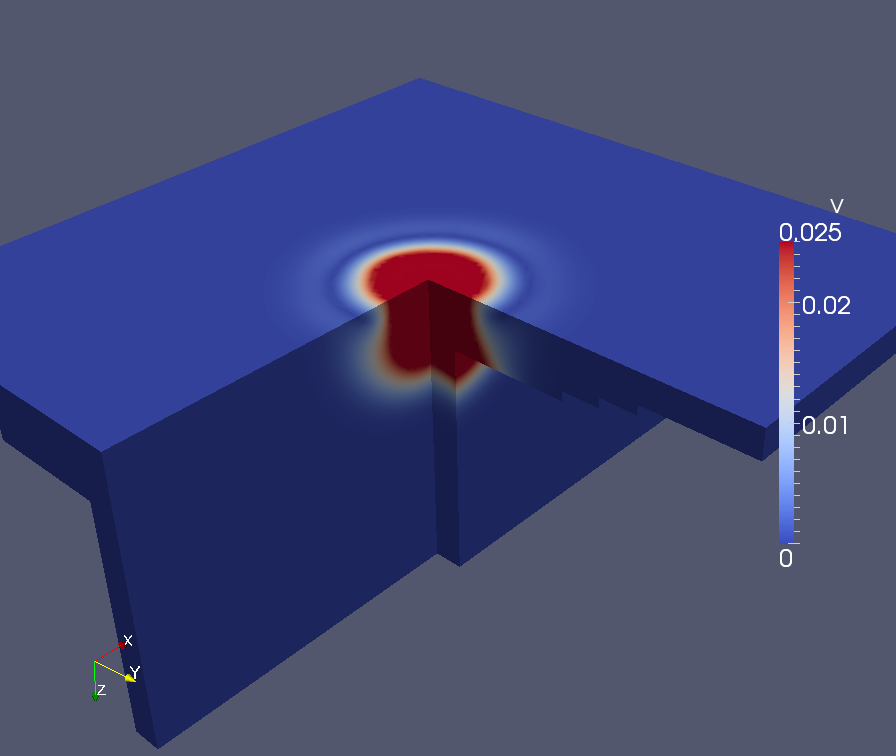
\includegraphics[width=\textwidth]{png/pkm-experiment/wing-stringer/wave-3d/v-0009.png}
\caption{5.5 мкс}
\end{subfigure}
\begin{subfigure}[b]{0.5\textwidth}
\centering
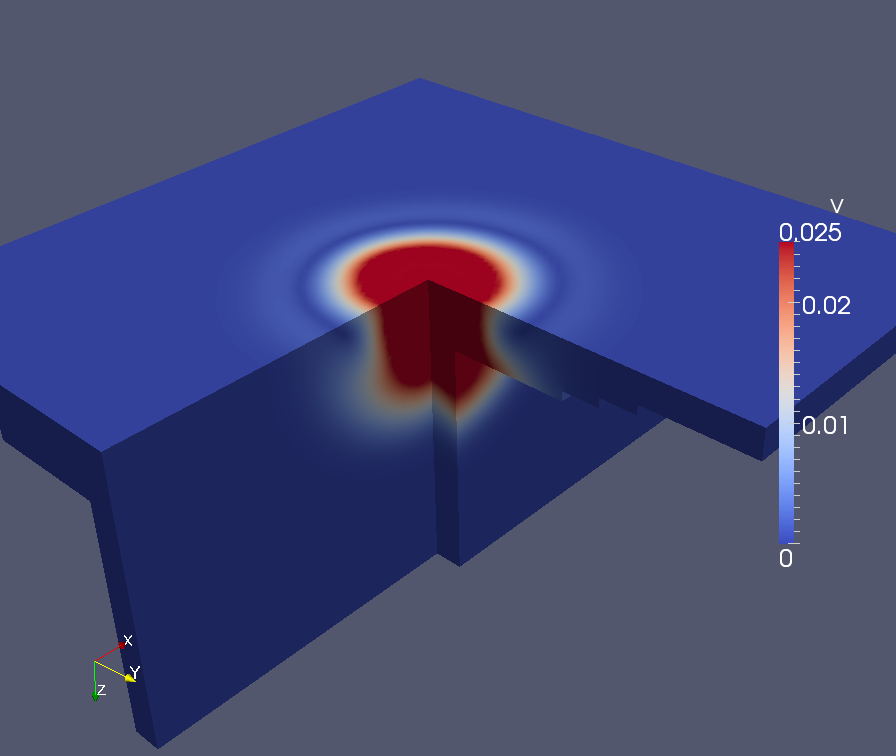
\includegraphics[width=\textwidth]{png/pkm-experiment/wing-stringer/wave-3d/v-0013.png}
\caption{8.0 мкс}
\end{subfigure}
\begin{subfigure}[b]{0.5\textwidth}
\centering
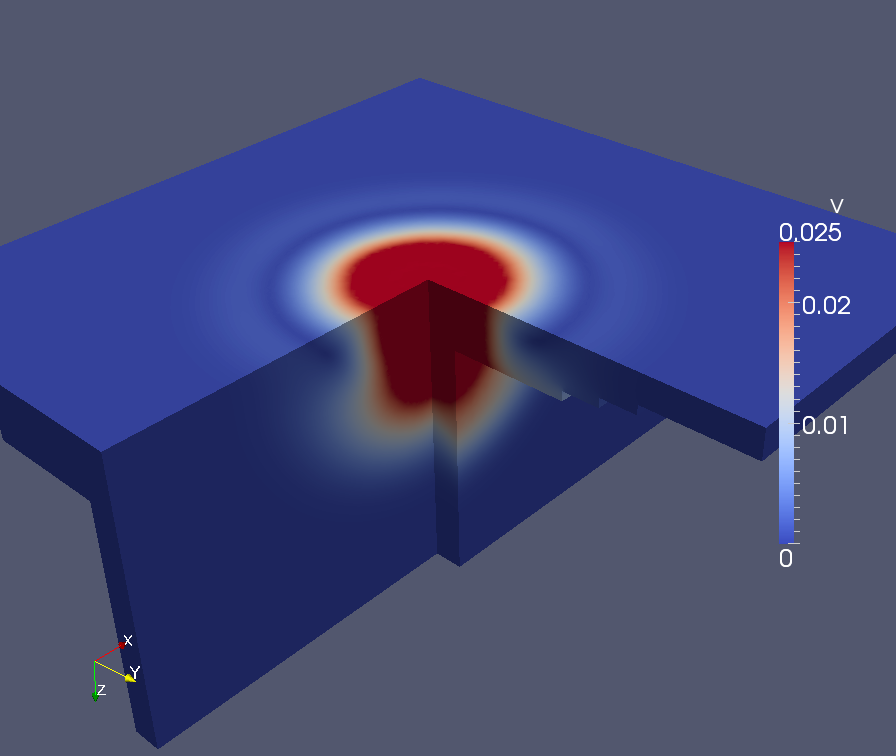
\includegraphics[width=\textwidth]{png/pkm-experiment/wing-stringer/wave-3d/v-0017.png}
\caption{10.5 мкс}
\end{subfigure}
\begin{subfigure}[b]{0.5\textwidth}
\centering
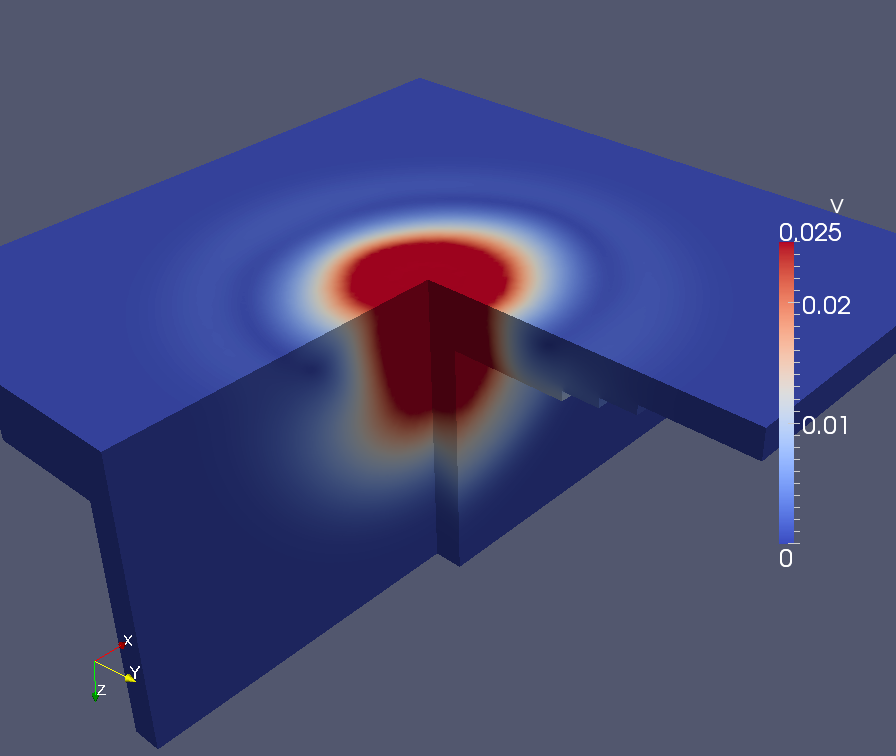
\includegraphics[width=\textwidth]{png/pkm-experiment/wing-stringer/wave-3d/v-0021.png}
\caption{13.0 мкс}
\end{subfigure}
\caption{Распространение возмущений в элементе обшивки и стрингере. Общая картина. Цветом показан модуль скорости.}
\label{pic:pkm_experiment_v3d_wing_stringer}
\end{figure}

\clearpage
\newpage

На рис. \ref{pic:pkm_experiment_stress_begin} - \ref{pic:pkm_experiment_stress_end} показано распространение напряжений в зоне удара.

В начальный момент (рис. \ref{pic:pkm_experiment_stress_begin}) фронт волны близок к сферическому, геометрические размеры определяются площадью контакта между ударником и пластиной, а точная форма -- строением элемента обшивки.

К концу данной стадии соударения волна сжатия проходит элемент обшивки. Для постановки без стрингера начинается отражение волны от противоположной свободной границы, фронт очевидным образом перестает быть сферическим, полная волновая картина в образце представляет сумму падающей и отражённой волн. Для постановки со стрингером начинается проникновение волны в стрингер. В данной области субпакеты, составляющие стрингер, ориентированы параллельно субпакетам обшивки (см. рис. \ref{pic:construction}), поэтому форма фронта не меняется.

\begin{figure}[htp]
\begin{subfigure}[b]{0.5\textwidth}
\centering
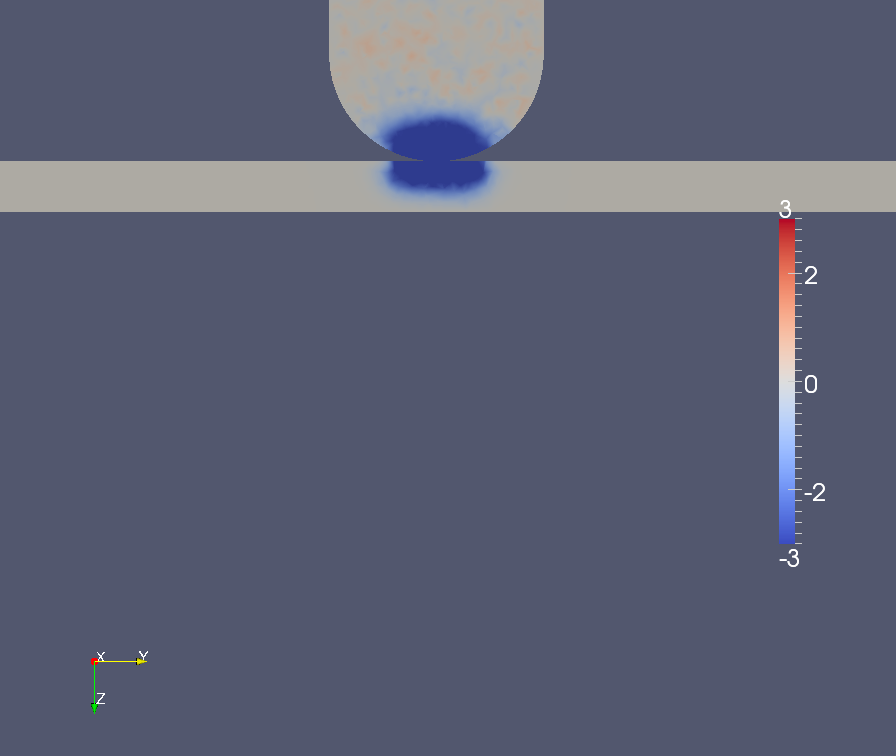
\includegraphics[width=\textwidth]{png/pkm-experiment/wing-only/wave/syy-0001.png}
\caption{0.5 мкс}
\end{subfigure}
\begin{subfigure}[b]{0.5\textwidth}
\centering
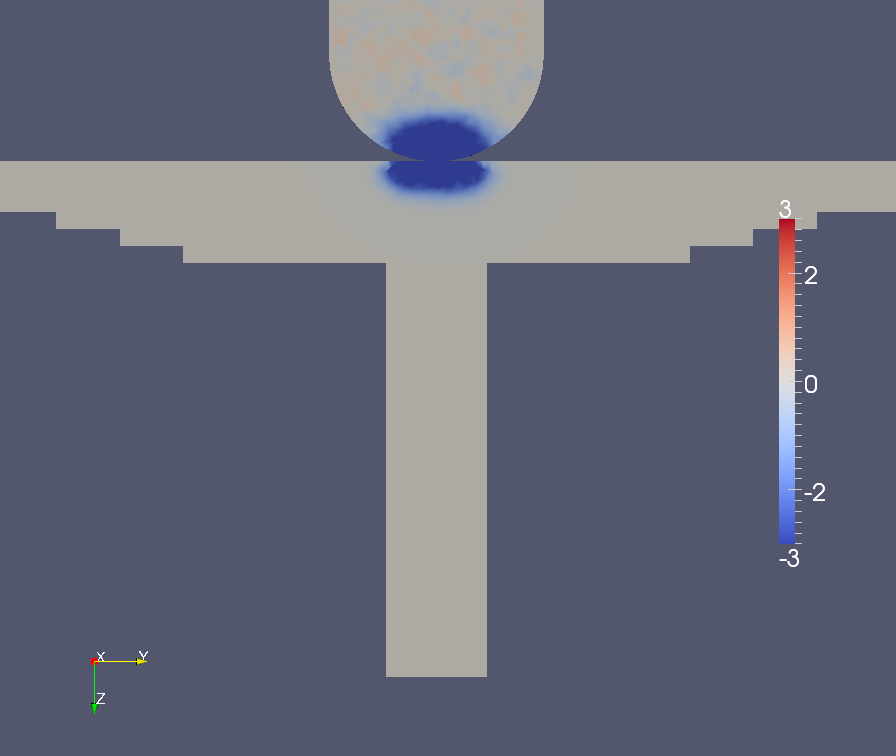
\includegraphics[width=\textwidth]{png/pkm-experiment/wing-stringer/wave/syy-0001.png}
\caption{0.5 мкс}
\end{subfigure}
\begin{subfigure}[b]{0.5\textwidth}
\centering
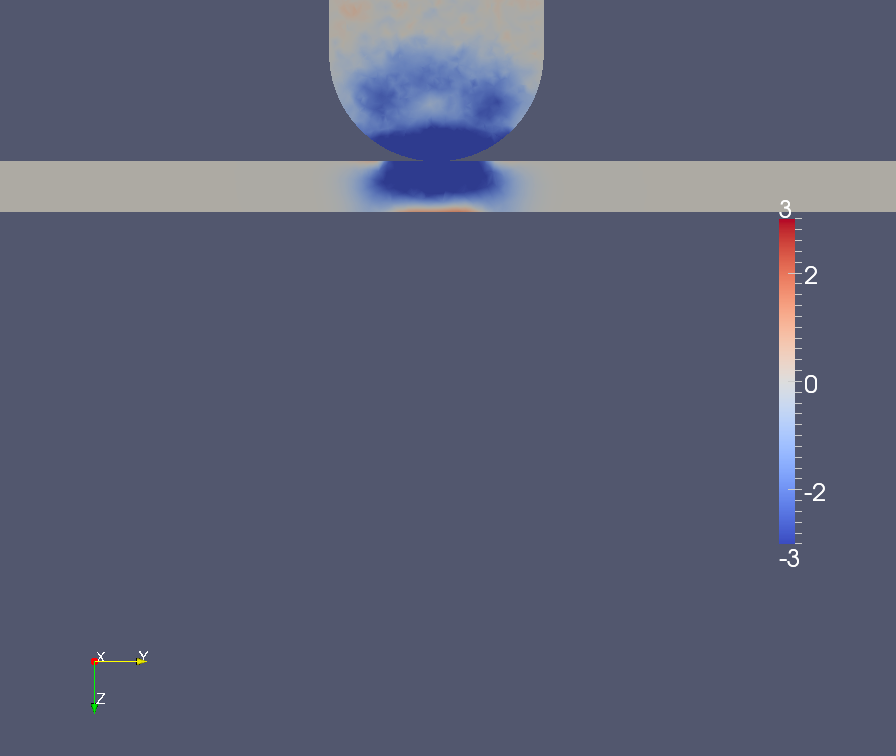
\includegraphics[width=\textwidth]{png/pkm-experiment/wing-only/wave/syy-0003.png}
\caption{3.0 мкс}
\end{subfigure}
\begin{subfigure}[b]{0.5\textwidth}
\centering
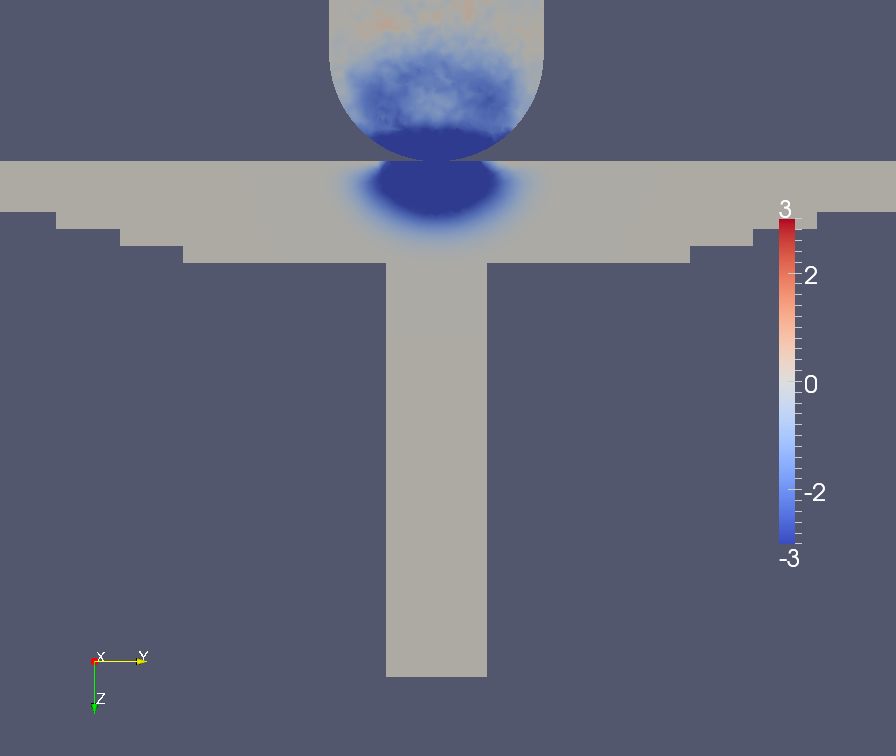
\includegraphics[width=\textwidth]{png/pkm-experiment/wing-stringer/wave/syy-0003.png}
\caption{3.0 мкс}
\end{subfigure}
\caption{Начальный момент удара. Цветом показаны напряжения. Синий соответствует сжатию, красный -- растяжению.}
\label{pic:pkm_experiment_stress_begin}
\end{figure}

На следующей стадии соударения (рис. \ref{pic:pkm_experiment_stress_middle}) в постановке без стрингера формируется волна растяжения, отражённая от свободной границы (рис. \ref{pic:pkm_experiment_stress_middle}а). Также заметно более слабая волна растяжения формируется в области, непосредственно прилежащей к зоне контакта (рис. \ref{pic:pkm_experiment_stress_middle}c и \ref{pic:pkm_experiment_stress_middle}d).

Для постановки со стрингером исходная волна сжатия еще не достигла свободной поверхности, от которой могло бы произойти заметное отражение. В результате наблюдаются менее выраженные области растяжения (рис. \ref{pic:pkm_experiment_stress_middle}b и \ref{pic:pkm_experiment_stress_middle}d), обусловленные волной растяжения в зоне контакта и относительно слабыми волнами, отражёнными от границ между субпакетами. На рис. \ref{pic:pkm_experiment_stress_middle}d видно изменение формы фронта первончальной волны. Это связано с тем, что волна дошла до зоны, где субпакеты стрингера ориентированы перпендикулярно субпакетам обшивки (см. рис. \ref{pic:construction}).

\begin{figure}[htp]
\begin{subfigure}[b]{0.5\textwidth}
\centering
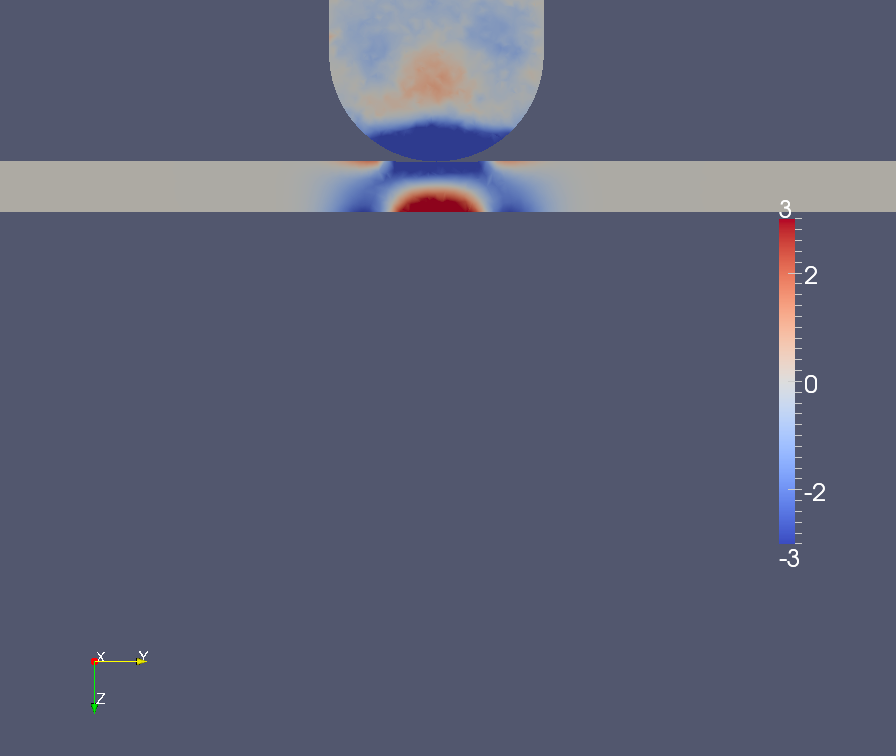
\includegraphics[width=\textwidth]{png/pkm-experiment/wing-only/wave/syy-0005.png}
\caption{5.5 мкс}
\end{subfigure}
\begin{subfigure}[b]{0.5\textwidth}
\centering
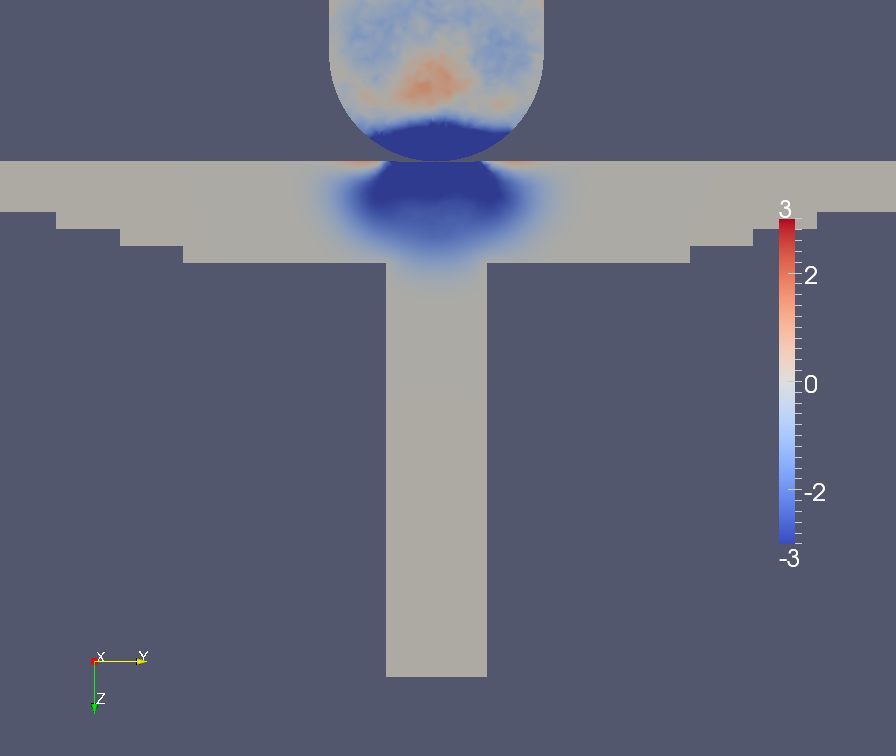
\includegraphics[width=\textwidth]{png/pkm-experiment/wing-stringer/wave/syy-0005.png}
\caption{5.5 мкс}
\end{subfigure}
\begin{subfigure}[b]{0.5\textwidth}
\centering
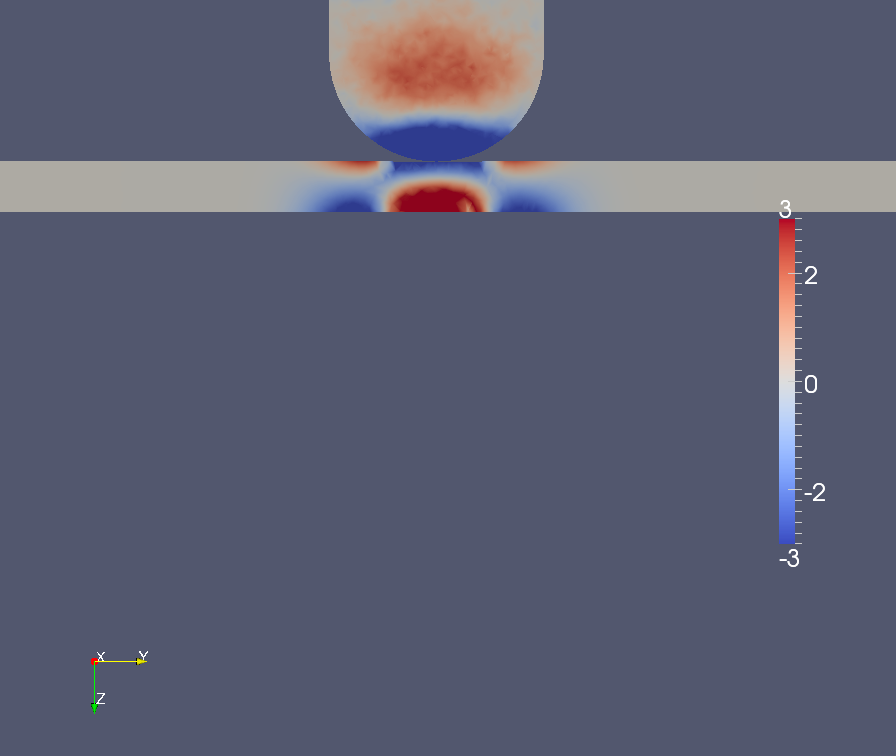
\includegraphics[width=\textwidth]{png/pkm-experiment/wing-only/wave/syy-0007.png}
\caption{8.0 мкс}
\end{subfigure}
\begin{subfigure}[b]{0.5\textwidth}
\centering
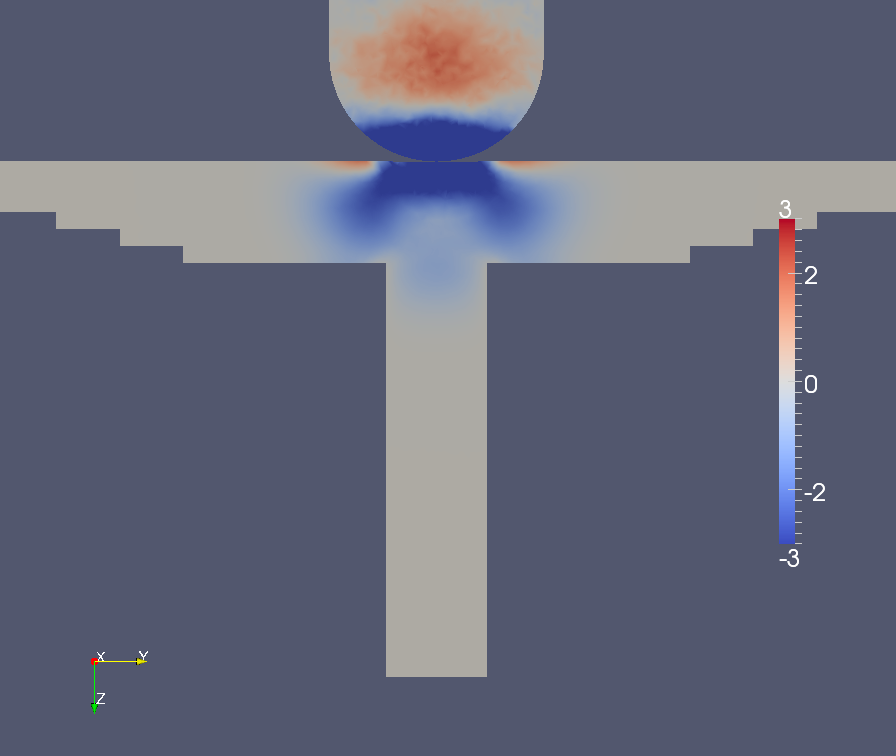
\includegraphics[width=\textwidth]{png/pkm-experiment/wing-stringer/wave/syy-0007.png}
\caption{8.0 мкс}
\end{subfigure}
\caption{Проникновение волны в конструкцию. Цветом показаны напряжения. Синий соответствует сжатию, красный -- растяжению.}
\label{pic:pkm_experiment_stress_middle}
\end{figure}

В дальнейшем в постановке без стрингера наблюдается многократное переотражение волн от параллельных свободных поверхностей и внутренних контактных границ. Одновременно с этим амплитуда волн затухает по мере удаления от места удара. Интерференция всех волн формирует распределение сжатий и растяжений (рис. \ref{pic:pkm_experiment_stress_middle}a, \ref{pic:pkm_experiment_stress_middle}c), характерное для удара по многослойной конструкции.

В постановке со стрингером происходит отражение волны от свободных поверхностей в районе изгиба субпакетов стрингера (рис. \ref{pic:pkm_experiment_stress_middle}b, \ref{pic:pkm_experiment_stress_middle}d). Отражение в целом заметно менее выражено, чем в постановке без стрингера. Это связано как с тем, что волна уже ослаблена отражением от контактных границ, так и геометрией области -- значительная часть энергии волны проходит в стрингер без взаимодействия со свободной границей.


\begin{figure}[htp]
\begin{subfigure}[b]{0.5\textwidth}
\centering
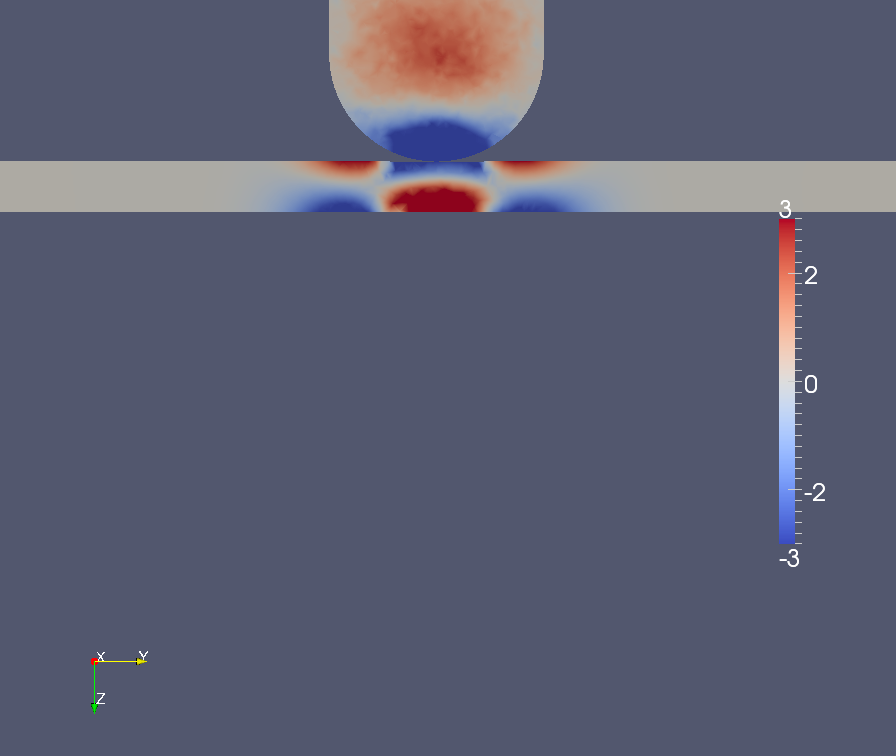
\includegraphics[width=\textwidth]{png/pkm-experiment/wing-only/wave/syy-0009.png}
\caption{10.5 мкс}
\end{subfigure}
\begin{subfigure}[b]{0.5\textwidth}
\centering
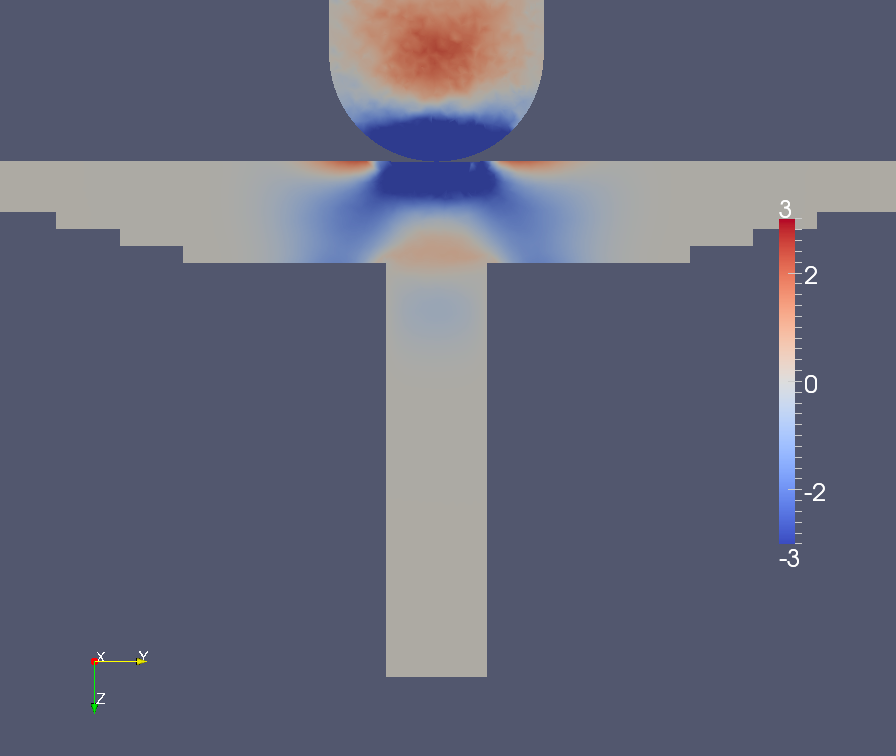
\includegraphics[width=\textwidth]{png/pkm-experiment/wing-stringer/wave/syy-0009.png}
\caption{10.5 мкс}
\end{subfigure}
\begin{subfigure}[b]{0.5\textwidth}
\centering
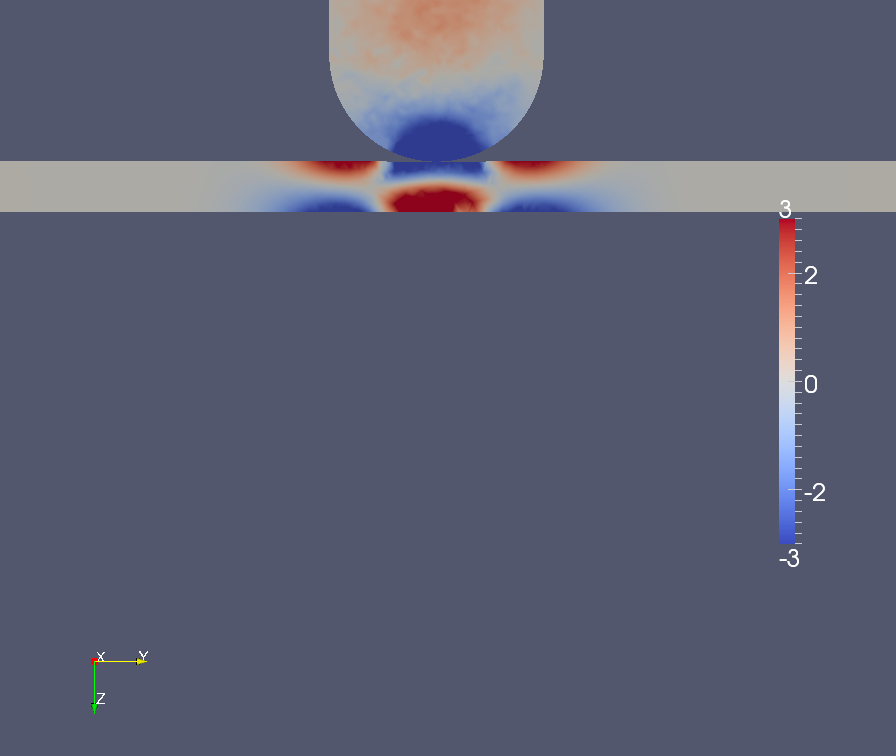
\includegraphics[width=\textwidth]{png/pkm-experiment/wing-only/wave/syy-0011.png}
\caption{13.0 мкс}
\end{subfigure}
\begin{subfigure}[b]{0.5\textwidth}
\centering
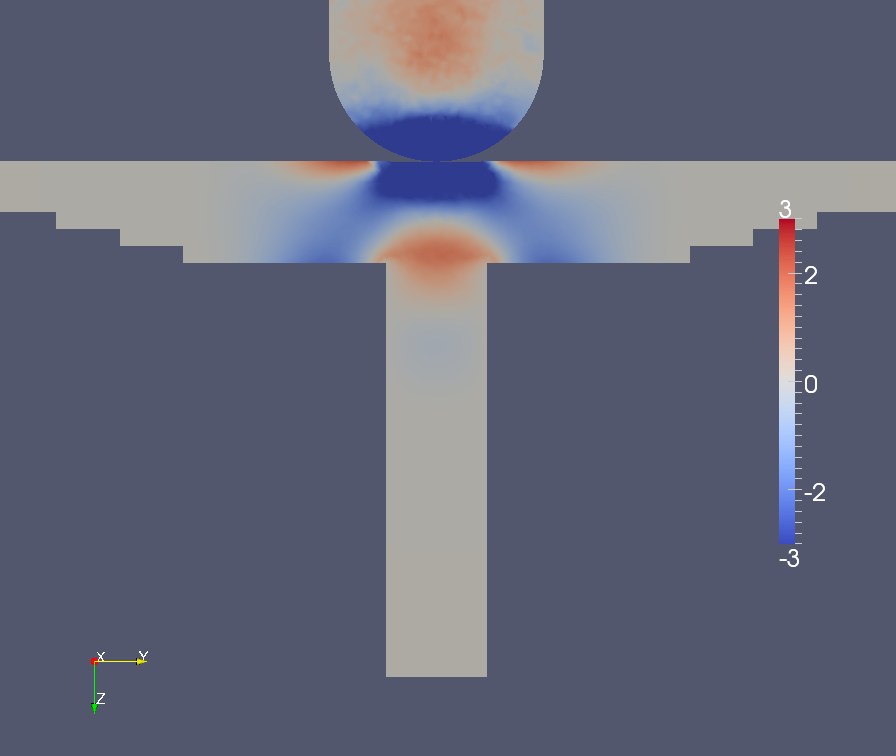
\includegraphics[width=\textwidth]{png/pkm-experiment/wing-stringer/wave/syy-0011.png}
\caption{13.0 мкс}
\end{subfigure}
\caption{Проникновение волны в конструкцию. Цветом показаны напряжения. Синий соответствует сжатию, красный -- растяжению.}
\label{pic:pkm_experiment_stress_end}
\end{figure}

\clearpage
\newpage

На рис. \ref{pic:pkm_experiment_compression} цветом показаны максимальные значения сжатия в каждой точке конструкции за все время соударения. Сжатия очевидным образом концентрируются в месте удара. Зона максимального сжатия имеет характерный размер порядка диаметра области контакта между ударником и пластиной.

\begin{figure}[htp]
\begin{subfigure}[b]{0.5\textwidth}
\centering
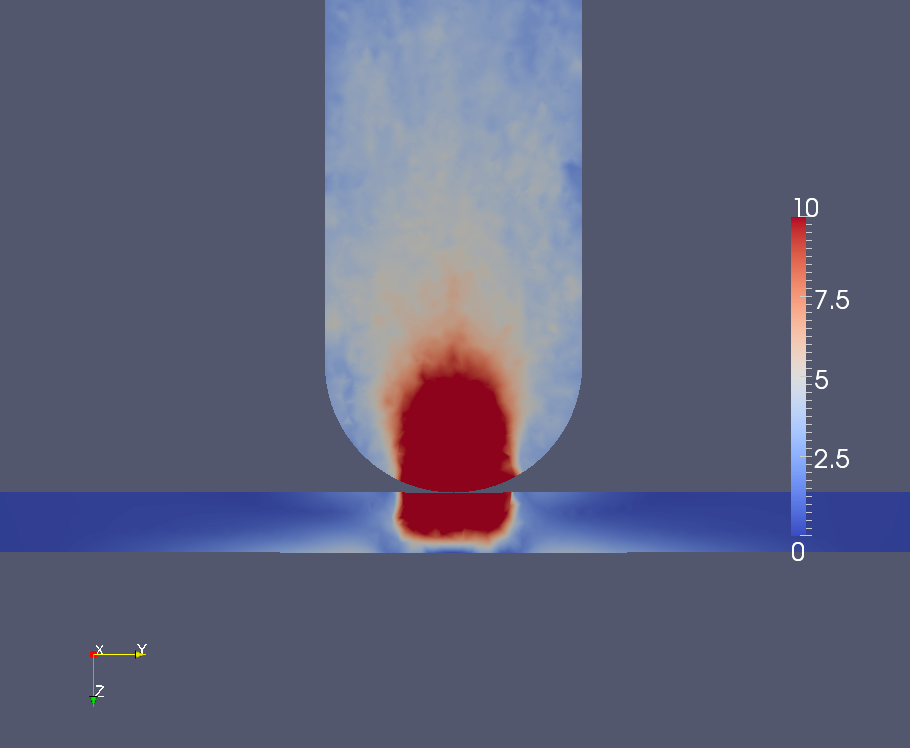
\includegraphics[width=\textwidth]{png/pkm-experiment/wing-only/compression.png}
\caption{Элемент обшивки.}
\end{subfigure}
\begin{subfigure}[b]{0.5\textwidth}
\centering
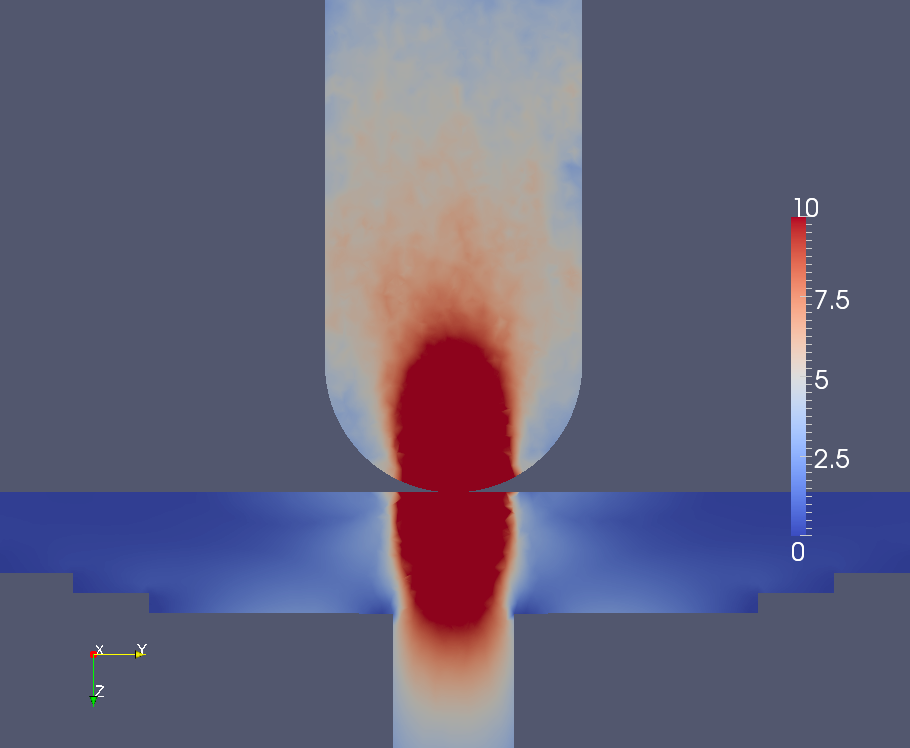
\includegraphics[width=\textwidth]{png/pkm-experiment/wing-stringer/compression.png}
\caption{Элемент обшивки и стрингер.}
\end{subfigure}
\caption{Максимальные сжатия (по модулю) за всё время соударения.}
\label{pic:pkm_experiment_compression}
\end{figure}

В случае конструкции без стрингера дополнительно видны относительно слабые области сжатия на обратной поверхности элемента обшивки, вызванные волнами, испытавшими два отражения -- первое от противолежащей свободной поверхности, второе от поверхности, по которой приходится удар.

В случае конструкции со стрингером видно заметное проникновение волны сжатия в основание стрингера. Вторичные зоны сжатия выражены значительно слабее, чем без стрингера, из-за большого количества переотражений от внутренних контактных границ.

Амплитуда максимального сжатия совпадает в обоих постановках. Диаметр зоны потенциальных разрушений составляет 16-20 мм.

Отдельно стоит отметить, что в субпакетах элемента обшивки сжатие действует поперёк волокон, а в основании стрингера -- вдоль волокон (см. рис. \ref{pic:construction}). Так как прочность монослоёв на сжатие в направлении волокон почти на порядок больше, чем поперёк них, то основные разрушения в конструкции стоит ожидать в элементе обшивки. В основании стрингера могут быть разрушены участки субпакетов, параллельные обшивке, но разрушение самого стрингера маловероятно.


\clearpage
\newpage

На рис. \ref{pic:pkm_experiment_tension} цветом показаны максимальные значения растяжения в каждой точке конструкции за все время соударения.

\begin{figure}[htp]
\begin{subfigure}[b]{0.5\textwidth}
\centering
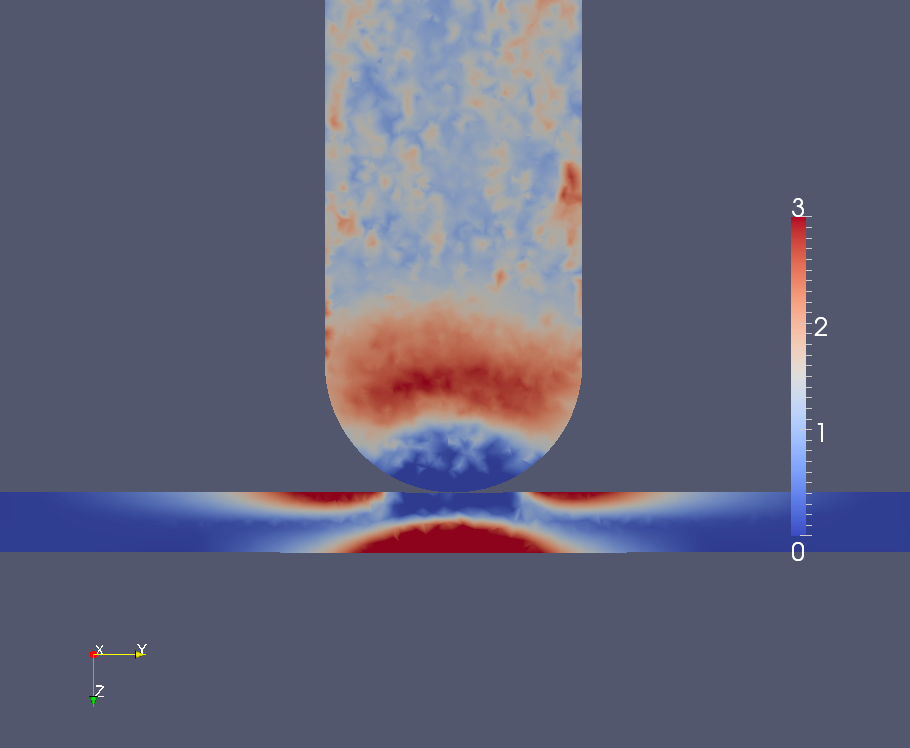
\includegraphics[width=\textwidth]{png/pkm-experiment/wing-only/tension.png}
\caption{Элемент обшивки.}
\end{subfigure}
\begin{subfigure}[b]{0.5\textwidth}
\centering
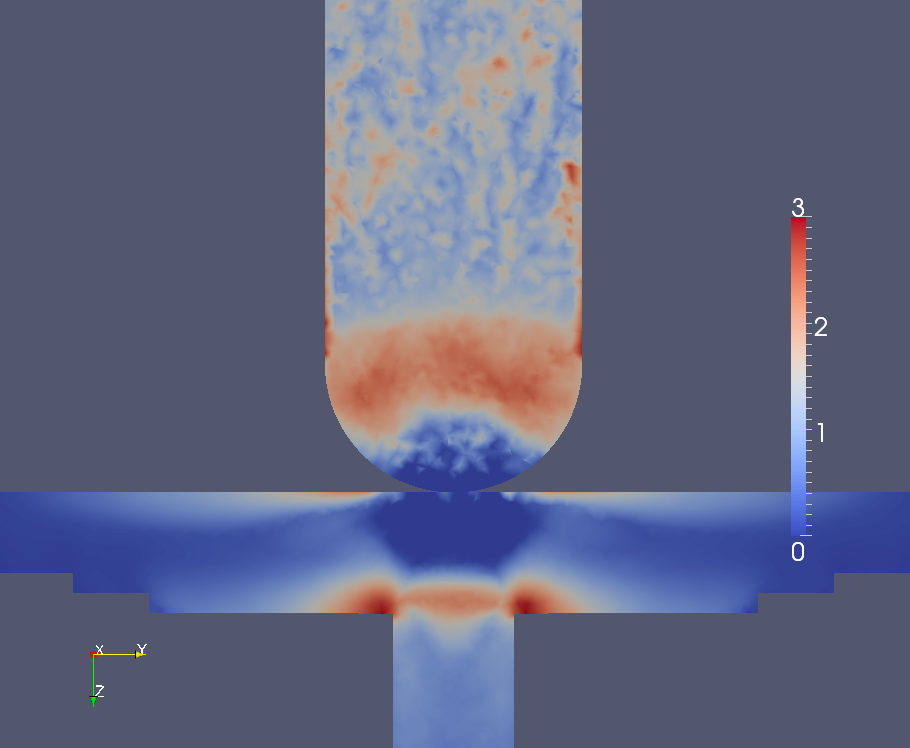
\includegraphics[width=\textwidth]{png/pkm-experiment/wing-stringer/tension.png}
\caption{Элемент обшивки и стрингер.}
\end{subfigure}
\caption{Максимальные растяжения (по модулю) за всё время соударения.}
\label{pic:pkm_experiment_tension}
\end{figure}

В случае конструкции без стрингера растягивающие напряжения выражены достаточно явно. Это связано с многократным переотражением волн в тонкой конструкции при относительно слабом рассеивании и затухании. Волны растяжения от первого и второго отражения имеют значительную амплитуду, что видно на рисунке.

Принципиально, что волны растяжения в обшивке действуют поперёк направления волокон в субпакетах обшивки. Сопротивление монослоёв такому типу нагрузки минимально. Диаметр зоны потенциальных разрушений оказывается заметно больше размеров ударника и составляет около 50 мм

В случае конструкции со стрингером столь ярко выраженные зоны растягивающих напряжений не формируются, так как волна нагрузки большей частью проходит в стрингер, который за счёт этого "разгружает" обшивку. У основания стрингера при отражении от свободных поверхностей формируются две зоны растягивающих напряжений -- в районе изгиба субпакетов стрингера и поперёк стрингера. В изгибе субпакетов напряжения достаточно велики и при этом действуют поперёк направления волокон. В этой зоне можно ожидать появления разрушений. Зона растяжения поперёк стрингера ориентирована таким образом, что нагрузка действует вдоль волокон, которые хорошо выдерживают такую нагрузку. В этой зоне разрушения маловероятны.


\clearpage
\newpage


На рис. \ref{pic:pkm_experiment_shear} цветом показаны максимальные значения сдвиговых напряжений в каждой точке конструкции за все время соударения.

\begin{figure}[htp]
\begin{subfigure}[b]{0.5\textwidth}
\centering
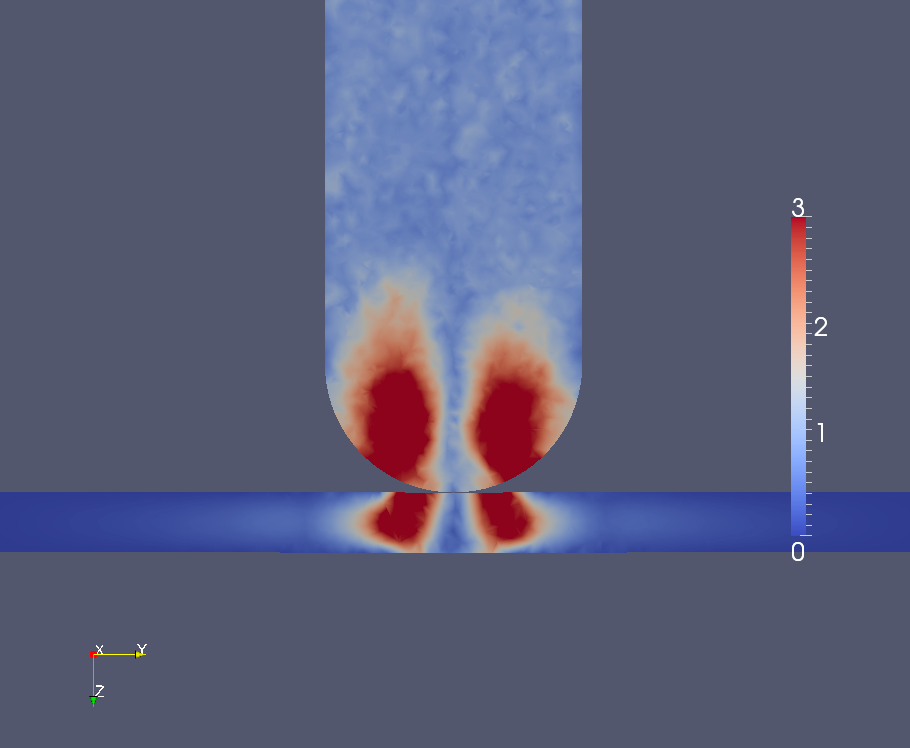
\includegraphics[width=\textwidth]{png/pkm-experiment/wing-only/shear.png}
\caption{Элемент обшивки.}
\end{subfigure}
\begin{subfigure}[b]{0.5\textwidth}
\centering
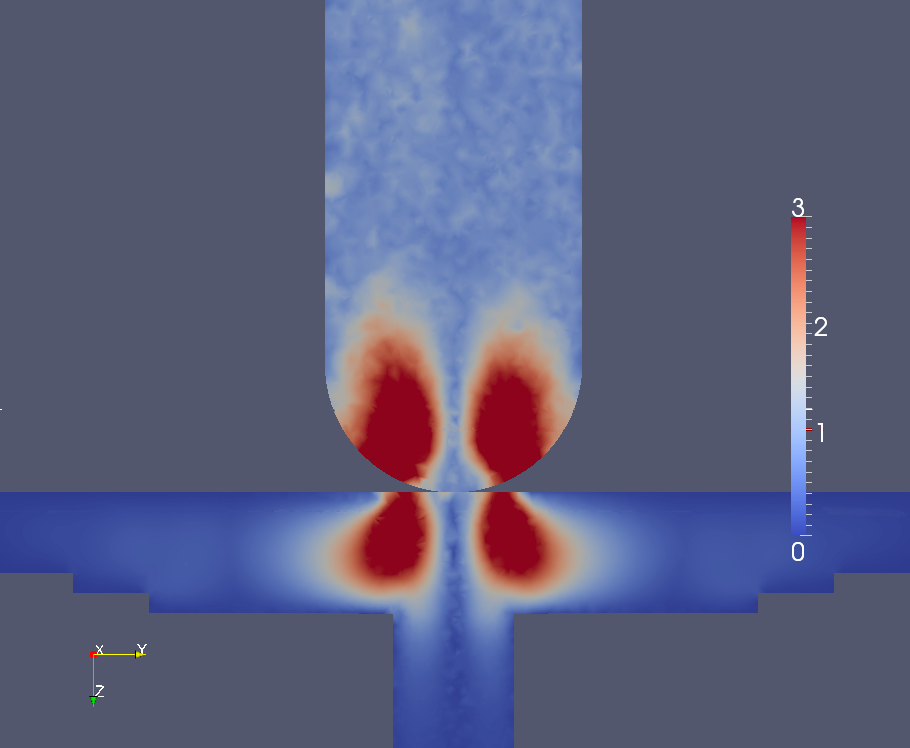
\includegraphics[width=\textwidth]{png/pkm-experiment/wing-stringer/shear.png}
\caption{Элемент обшивки и стрингер.}
\end{subfigure}
\caption{Максимальные сдвиговые напряжения (по модулю) за всё время соударения.}
\label{pic:pkm_experiment_shear}
\end{figure}

Сдвиговые напряжения локализуются на периферии зоны максимального сжатия. В однородной среде зона максимальных сдвиговых напряжений имеет форму конуса, расходящегося от места удара (см. рис. \ref{pic:destruction_test}). В случае многослойной среды, моделирующей композит, из-за переотражений волн формируется зона, по форме более близкая к колоколу. Вследствие этого характерный размер зоны действия сдвиговых напряжений зависит от толщины пластины.

На качественном уровне картина оказывается одинаковой как для одиночного элемента обшивки, так и для элемента обшивки со стрингером. Количественно размер повреждённой зоны оказывается несколько больше во втором случае из-за большей толщины конструкции в месте удара. Для первой постановки характерный размер зоны составляет 20 мм, для второй -- 25-30 мм.

Во всей области действия максимальных сдвиговых нагрузок структура композита такова, что направление сдвига приходится поперёк волокон. Монослои композита не очень хорошо держат нагрузку такого вида, поэтому разрушения в данной области возможны.


\clearpage
\newpage


На рис. \ref{pic:pkm_experiment_mises} цветом показаны максимальные значения эквивалентного напряжения Мизеса в каждой точке конструкции за все время соударения.

\begin{figure}[htp]
\begin{subfigure}[b]{0.5\textwidth}
\centering
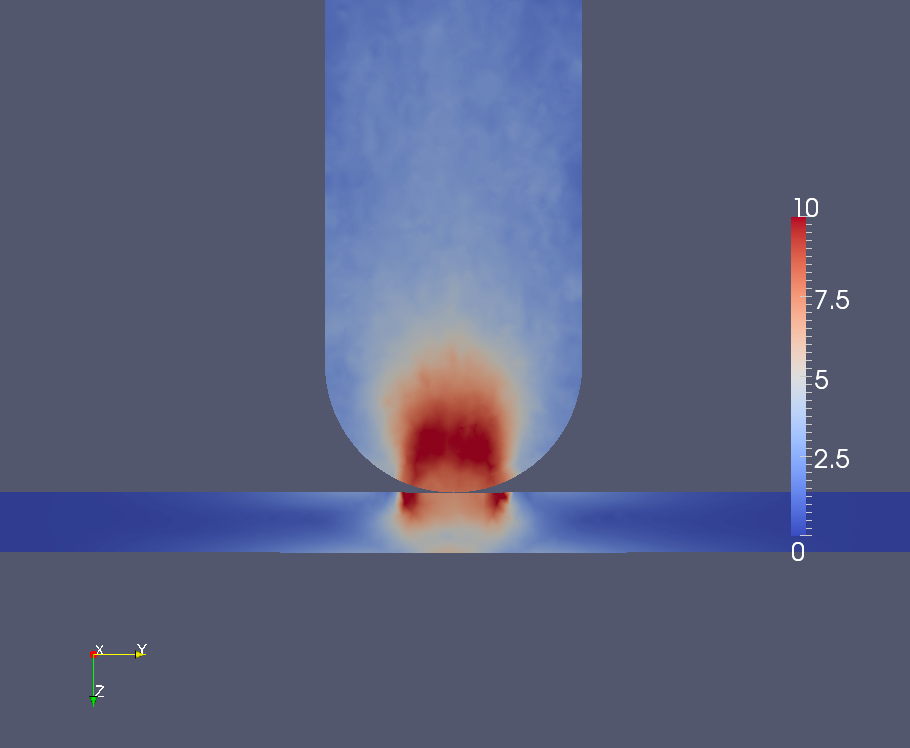
\includegraphics[width=\textwidth]{png/pkm-experiment/wing-only/mises.png}
\caption{Элемент обшивки.}
\end{subfigure}
\begin{subfigure}[b]{0.5\textwidth}
\centering
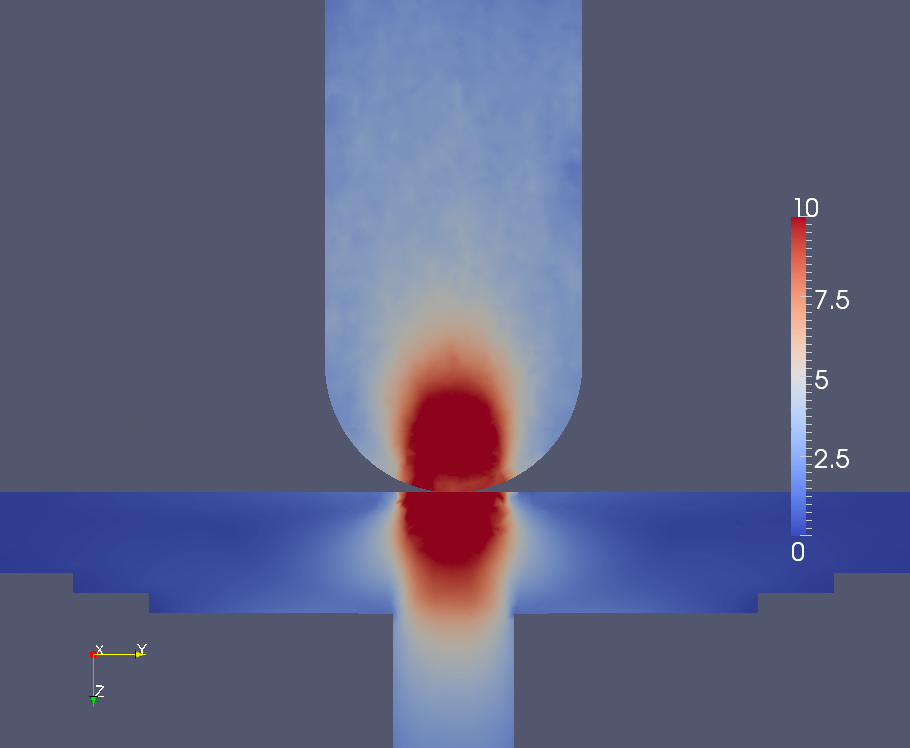
\includegraphics[width=\textwidth]{png/pkm-experiment/wing-stringer/mises.png}
\caption{Элемент обшивки и стрингер.}
\end{subfigure}
\caption{Максимальное эквивалентное напряжение Мизеса (по модулю) за всё время соударения.}
\label{pic:pkm_experiment_mises}
\end{figure}

Как рассмотрено выше, напряжение Мизеса характеризует девиаторную часть тензора напряжений. Нагрузки такого типа связаны с изменением формы вещества без изменения его объёма. В однородной среде зона максимальных напряжений Мизеса с хорошей точностью совпадает с зоной максимальных сдвиговых напряжений (см. рис. \ref{pic:destruction_test}) и так же как и она имеет форму конуса, хотя и несколько большего и с более ярко выраженным максимумом в точке удара.

Для композита рассматриваемой структуры получено, что характер распределения напряжений Мизеса несколько меняется. Область принимает колоколообразную форму, аналогично сдвиговым напряжениям. Кроме того, значительно более ярко по сравнению с изотропной средой выражен максимум непосредственно в зоне удара.

В постановке без стрингера напряжения Мизеса значительно меньше, чем при наличии стрингера, так как отражения от близкой свободной поверхности быстро компенсируют девиаторную часть нагрузки, переводя её в растяжения.


\clearpage
\newpage


Для оценки итоговых областей разрушений необходимо учитывать разрушения всех приведённых типов. При этом, как видно из таблицы \ref{tbl:max_stresses}, устойчивость монослоёв при нагрузках разных типов значительно отличается. В качестве интегральной характеристики воздействия использовался параметр

\begin{equation}
\sigma^* = \sum{k_i max(\sigma_i)},
\end{equation}

где суммирование ведётся по типам нагрузки (сжатие, растяжение, сдвиг, изменение формы), $max(\sigma_i)$ -- максимальное значение напряжения данного типа в данной точке за всё время воздействия, $k_i$ -- коэффициент нормировки. Коэффициенты нормировки $k_i$ для напряжений различных типов были выбраны обратно пропорционально пределу прочности монослоёв при нагрузках соответствующего типа. Для упрощения оценки использовались следующие значения: сжатие -- 1, сдвиг и изменение формы -- 2, растяжение -- 3.

Вообще говоря, в случае динамической нагрузки пределы прочности могут заметно отличаться от указанных значений. Соответственно, следует корректировать и вклад напряжений разных типов в итоговое распределение разрушений. Тем не менее, для низкоскоростного удара воспользуемся этими данными.

Интегральная оценка областей потенциального разрушения материала для постановки с отдельным элементом обшивки приведена на рис. \ref{pic:pkm_experiment_wing_only_result}. Размер разрушенной области заметно превышает размер ударника и составляет 50-60 мм. По форме разрушенная область представляет собой цилиндр с утоньшением посередине. Как было показано выше, разрушения на оси удара (10-15 мм от оси симметрии удара) связаны со сжатием и сдвигом. Разрушения в более дальней области (15-30 мм от оси симметрии удара) обусловлены волнами растяжения.


\begin{figure}[htp]
\begin{subfigure}[b]{\textwidth}
\centering
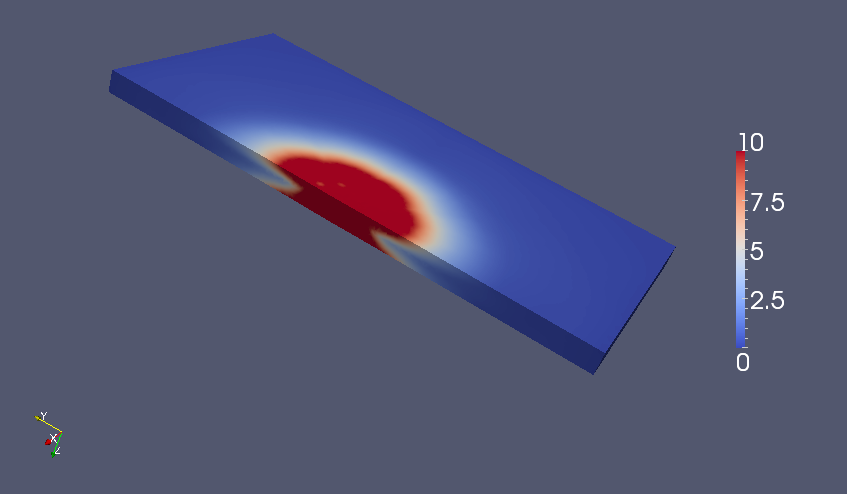
\includegraphics[width=\textwidth]{png/pkm-experiment/wing-only/sum-3d.png}
\caption{Срез через центр элемента параллельно грани.}
\end{subfigure}
\begin{subfigure}[b]{\textwidth}
\centering
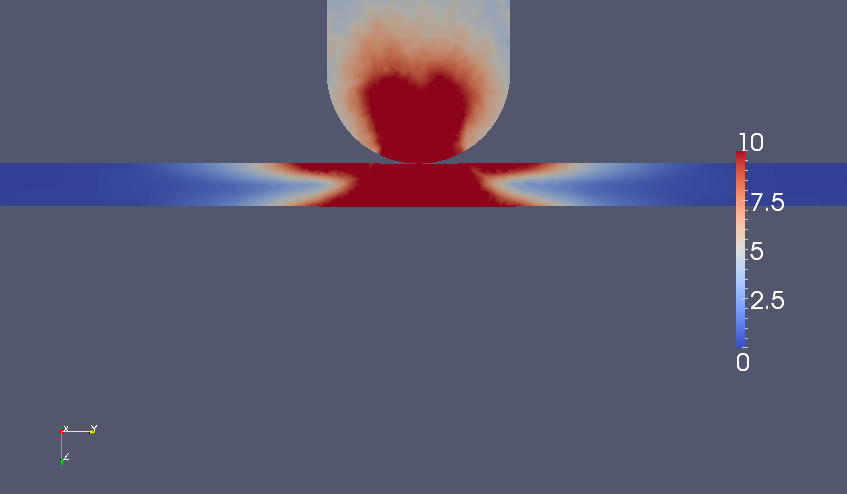
\includegraphics[width=\textwidth]{png/pkm-experiment/wing-only/sum.png}
\caption{Сечение через центр элемента параллельно грани.}
\end{subfigure}
\caption{Области разрушений в элементе обшивки.}
\label{pic:pkm_experiment_wing_only_result}
\end{figure}

Интегральная оценка областей потенциального разрушения материала для постановки с элементом обшивки и стрингером приведена на рис. \ref{pic:pkm_experiment_wing_stringer_result}. Размер разрушенной области порядка размера ударника -- 25 мм. По форме разрушенная область представляет собой колокол, уходящий вглубь конструкции. Как было показано выше, разрушения обусловлены сжатием, сдвигом и изменением формы.

Отдельный комментарий необходим относительно отмеченной области разрушения в стрингере. Значения напряжений в данной области действительно достаточно велики, однако воздействие направлено вдоль волокон (см. рис. \ref{pic:construction}. Предел прочности в направлении волокон монослой выдерживает практически на порядок лучше, чем поперёк волокон (\ref{tbl:max_stresses}), поэтому на практике разрушения в стрингере маловероятны.

\begin{figure}[htp]
\begin{subfigure}[b]{\textwidth}
\center
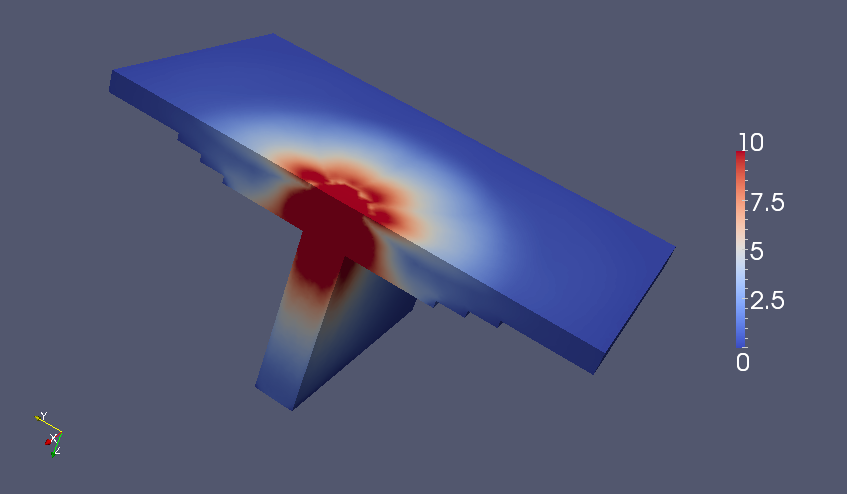
\includegraphics[width=\textwidth]{png/pkm-experiment/wing-stringer/sum-3d.png}
\caption{Срез через центр элемента параллельно грани.}
\end{subfigure}
\begin{subfigure}[b]{\textwidth}
\center
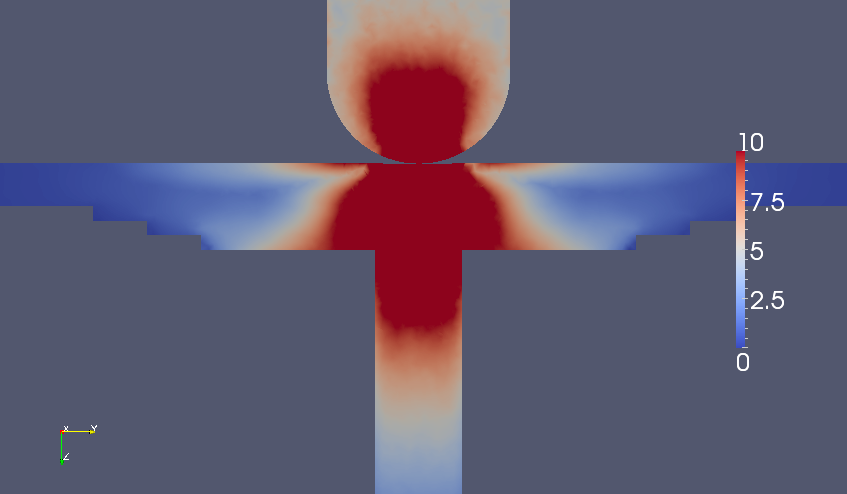
\includegraphics[width=\textwidth]{png/pkm-experiment/wing-stringer/sum.png}
\caption{Сечение через центр элемента параллельно грани.}
\end{subfigure}
\caption{Области разрушений в элементе обшивки и стрингере.}
\label{pic:pkm_experiment_wing_stringer_result}
\end{figure}

Таким образом, в случае динамического воздействия разрушения в конструкции со стрингером оказываются заметно меньше за счёт того, что волны напряжения уходят в стрингер, и это "разгружает" элемент обшивки. Данный факт отдельно интересен в связи с тем, что при статической нагрузке наличие стрингера напротив приводит к концентрации напряжений и более раннему разрушению элемента обшивки.


\clearpage
\newpage


Дополнительно были выполнены расчёты для несимметричного удара по элементу обшивки со стрингером. Вид расчётной области представлен на рис. \ref{pic:wing_stringer_non_center_scene}. Точка удара в этой постановке смещена от оси прикрепления стрингера на 30 мм перпендикулярно плоскости стрингера. Все остальные параметры объектов без изменений.

\begin{figure}[htp]
\center{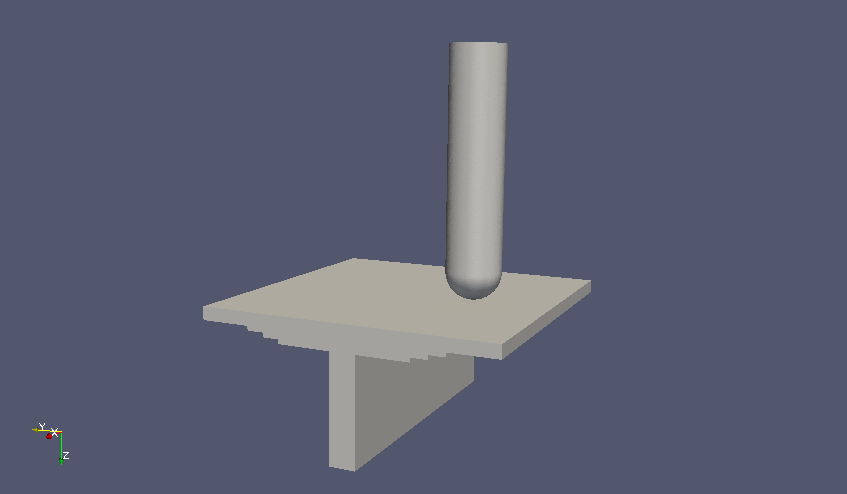
\includegraphics[width=0.75\textwidth]{png/pkm-experiment/wing-stringer-non-center/scene.png}}
\caption{Несимметричный удар по элементу обшивки со стрингером. Вид расчетной области.}
\label{pic:wing_stringer_non_center_scene}
\end{figure}

Данная постановка интересна по двум причинам. Во-первых, в ходе эксплуатации композитных изделий следует ожидать по большей части несимметричных ударов. Во-вторых, сравнение результатов воздействия при центральном и нецентральном ударах по конструкции со стрингером позволяет выполнить верификацию полученных результатов и уточнить, какие типы нагрузок преимущественно вызывают разрушения.

Полученные значения максимальных напряжений представлены на рис. \ref{pic:pkm_experiment_non_center}. Распределение максимальных сжатий, сдвигов и напряжений Мизеса хорошо совпадает с аналогичными распределениями для удара по элементу обшивки без стрингера. Этот результат вполне логичен, так как общий вид конструкции тот же -- тонкая пластина, в которой наблюдаются множественные переотражения на малой толщине. Детали геометрии области отличаются -- больше толщина и больше контактных границ, обратная свободная поверхность не плоская. Это влияет на точную форму волновых фронтов, но не меняет принципиальную картину. Стрингер расположен в стороне от зоны удара и не разгружает конструкцию, так как наиболее сильные волны до него не доходят, а диссипация слабых многократно отражённых и преломлённых волн не сказывается на зонах потенциальных разрушений.

\clearpage
\newpage

\begin{figure}[h]
\begin{subfigure}[b]{0.5\textwidth}
\centering
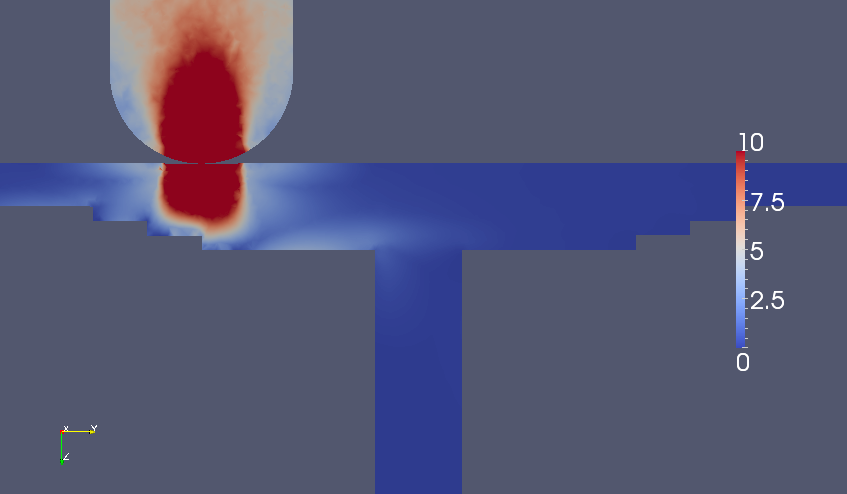
\includegraphics[width=\textwidth]{png/pkm-experiment/wing-stringer-non-center/compression.png}
\caption{Максимальное сжатие (по модулю) за всё время соударения.}
\end{subfigure}
\begin{subfigure}[b]{0.5\textwidth}
\centering
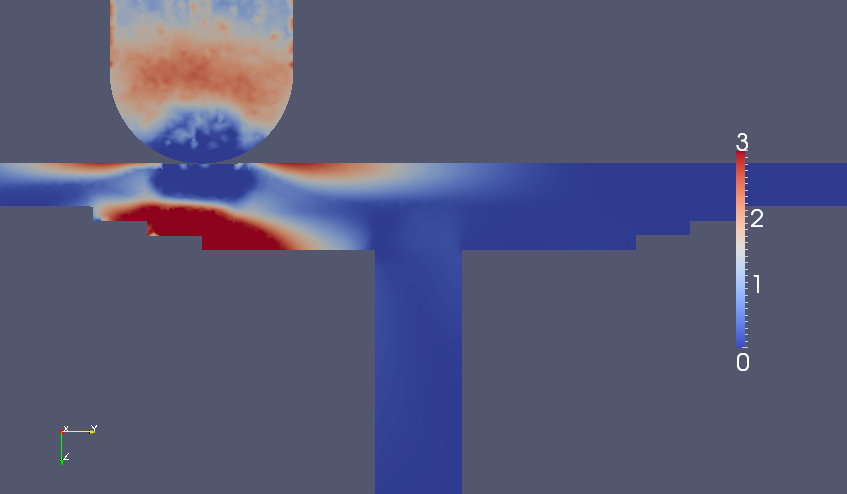
\includegraphics[width=\textwidth]{png/pkm-experiment/wing-stringer-non-center/tension.png}
\caption{Максимальное растяжение (по модулю) за всё время соударения.}
\end{subfigure}
\begin{subfigure}[b]{0.5\textwidth}
\centering
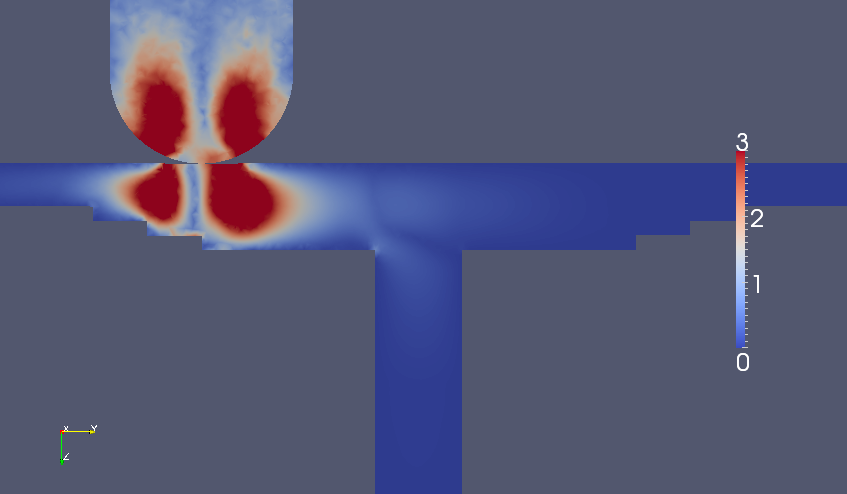
\includegraphics[width=\textwidth]{png/pkm-experiment/wing-stringer-non-center/shear.png}
\caption{Максимальное сдвиговое напряжение (по модулю) за всё время соударения.}
\end{subfigure}
\begin{subfigure}[b]{0.5\textwidth}
\centering
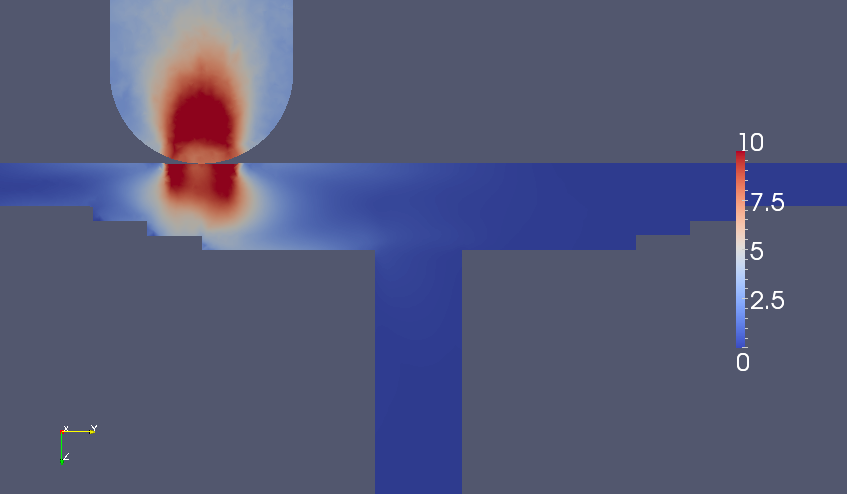
\includegraphics[width=\textwidth]{png/pkm-experiment/wing-stringer-non-center/mises.png}
\caption{Максимальное напряжение Мизеса (по модулю) за всё время соударения.}
\end{subfigure}
\caption{Максимальные нагрузки при нецентральном ударе.}
\label{pic:pkm_experiment_non_center}
\end{figure}

Иначе обстоит дело для волн растяжения -- их распределение принципиально отличается от рассмотренных постановок с центральными ударами.

В рассматриваемой постановке зона контакта ударника и пластины находится напротив края крепления стрингера. Первоначальная волна сжатия отражается как от тыльных поверхностей субпакетов (параллельных внешней поверхности обшивки), так и от кромок субпакетов стрингера (расположенных перпендикулярно к поверхности обшивки). В результате каждого такого отражения формируется волна растяжения. Три такие волны движутся вверх, и три -- вправо. При сложении этих волн формируется итоговая область растягивающих напряжений (рис. \ref{pic:pkm_experiment_non_center}b).

Амплитуда растягивающих напряжений в области края крепления стрингера из-за сложения волн оказывается в 2.5 раза больше, чем значение на тыльной поверхности для конструкции без стрингера. При этом на верхней границе образца растягивающие напряжения оказываются заметно меньше (в 1.5-2 раза) по сравнению с элементом обшивки без стрингера.

Интегральная оценка воздействия и потенциальные зоны разрушения при нецентральном ударе показаны на рис. \ref{pic:pkm_experiment_wing_stringer_non_center_result}. Форма области близка к колоколу, но при этом является достаточно узкой -- её диаметр не превышает диаметра ударника и составляет 20-25 мм.


\begin{figure}[h]
\begin{subfigure}[b]{\textwidth}
\center
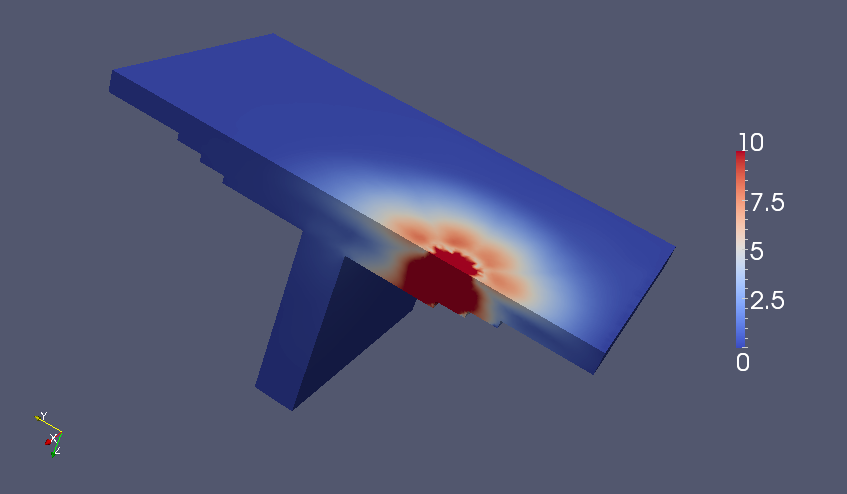
\includegraphics[width=\textwidth]{png/pkm-experiment/wing-stringer-non-center/sum-3d.png}
\caption{Срез через центр элемента параллельно грани.}
\end{subfigure}
\begin{subfigure}[b]{\textwidth}
\center
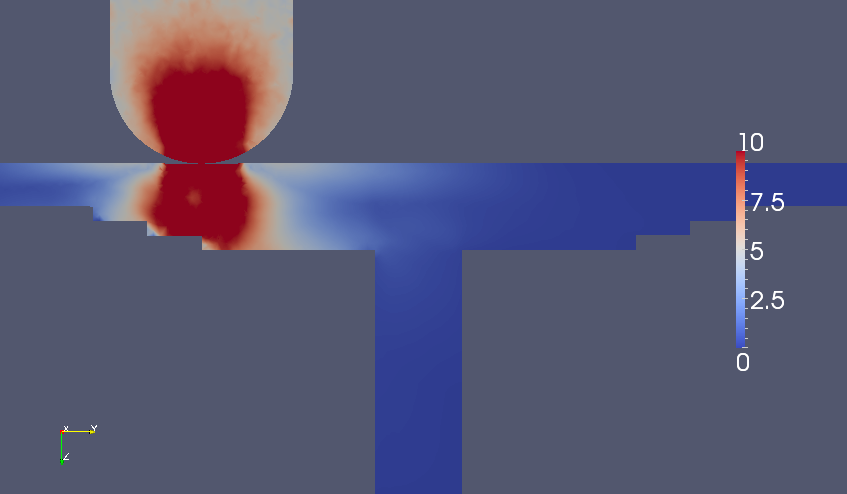
\includegraphics[width=\textwidth]{png/pkm-experiment/wing-stringer-non-center/sum.png}
\caption{Сечение через центр элемента параллельно грани.}
\end{subfigure}
\caption{Области разрушений при нецентральном ударе.}
\label{pic:pkm_experiment_wing_stringer_non_center_result}
\end{figure}


Основные результаты в части разрушения конструкции представлены в таблице \ref{tbl:destruction_summary}.

\begin{table}
\centering
\begin{tabular}{|c|c|c|}
\hline
Постановка задачи & Диаметр разрушенной области, мм & Чем обусловлено разрушение \\
\hline
Элемент обшивки без стрингера, центральный удар & 50-60 & Сжатие и сдвиг в центральной зоне, растяжение в периферийной зоне \\
Элемент обшивки со стрингером, центральный удар & 25-30 & Сжатие, сдвиг, напряжение Мизеса \\
Элемент обшивки со стрингером, нецентральный удар & 20-25 & Сжатие и сдвиг на внешней поверхности, растяжение на тыльной поверхности \\
\hline
\end{tabular}
\caption{Прочностные характеристики монослоёв.}
\label{tbl:destruction_summary}
\end{table}



\clearpage
\newpage


\section{Взаимодействие падающей волны с поврежденной зоной}

Отдельной задачей является моделирование тела с повреждениями. Данная задача важна при определении последствий повторных ударов по конструкции. В этом случае конструкция может уже не являться сплошной, в ней содержатся трещины, зоны раздробленного материала и другие повреждения.

Реологические характеристики поврежденных зон заметно отличаются от характеристик окружающего материала. С одной стороны, это приводит к тому, что остаточная прочность конструкции может заметно снизиться по сравнению с первоначальной. С другой стороны, появившиеся неоднородности оказывают влияние на волновую картину при повторных воздействиях и могут заметно ее искажать.

В данной работе рассматривается взаимодействие волны нагрузки с зоной разрушенного материала. Расчетная область с сеткой представлена на рис. \ref{pic:crack_mesh}. Разрушенная зона и окружающий неповрежденный материал моделируются явным образом на отдельных сетках. На контактной границе стоит условие полного слипания.

\begin{figure}[htp]
\center{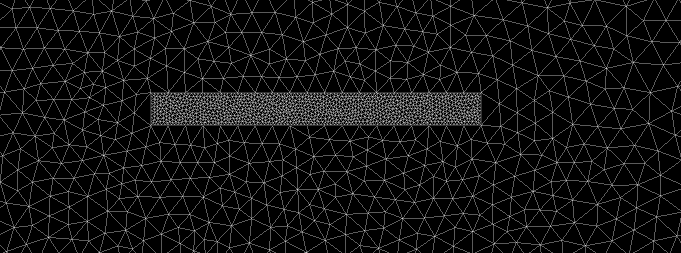
\includegraphics[width=0.5\textwidth]{png/wave-around-crack/mesh.png}}
\caption{Расчетная область с сеткой.}
\label{pic:crack_mesh}
\end{figure}

Материал исходной среды принимается хрупким, что соответствует эпоксидной матрице композита. В этом случае разрушенная зона представляет собой раздробленный материал. Через зону разрушения такого типа продольные волны проходят медленнее, чем через окружающую неповрежденную среду, а поперечные волны практически не проходят. В связи с этим раздробленная зона моделируется изменением характеристик материала - параметр $\lambda$ уменьшается в два раза, параметр $\mu$ принимается близким к нулю. 

Характеристики исходного и разрушенного материала приведены в табл. \ref{tbl:crack}
\begin{table}
\centering
\begin{tabular}{|c|c|c|c|c|c|}
\hline
Материал & $\rho$, кг/м$^{3}$ & $\lambda$, ГПа & $\mu$, ГПа &
$c_p$, м/с & $c_s$, м/с \\
\hline
Матрица (эпоксидная смола) & 1250 & 1.44 & 0.96 & 1640 & 876 \\
Разрушенная матрица & 1250 & 0.73 & 0.01 & 775 & 89 \\
\hline
\end{tabular}
\caption{Характеристики исходного и разрушенного материала.}
\label{tbl:crack}
\end{table}

Разрушенная область имеет малые размеры по сравнению с полной конструкцией, что требует использовать в ней крайне мелкую сетку. Использование сетки такой же мелкости для расчета всего окружающего материала ведет к резкому увеличению требуемого объема как оперативной памяти в ходе расчёта, так и места на диске для сохранения результатов.

В связи с этим кажется разумным использовать сетки разной мелкости - более мелкую в малой разрушенной области и более грубую в неразрушенном окружающем материале. Очевидно, что при этом точность решения в окружающей среде будет ниже, но в большинстве случаев это приемлемо. Более тонким вопросом является расчёт контактной границы в случае сеток разной мелкости. Описанный алгоритм с использованием виртуальных узлов позволяет считать контактную границу между сетками любой мелкости, но точность при этом, очевидно, будет определяться интерполяцией виртуальных узлов на более грубой сеткой.

Для тестирования совместного использования сеток разной мелкости было выполнено два расчёта. В первом расчёте мелкость сеток одинакова для разрушенной области и окружающего материала - используется мелкая сетка, размер элементов выбирается таким образом, чтобы на толщине разрушенной области (минимальный характерный размер задачи) было около десяти ячеек. Во втором расчёте используются сетки разной мелкости - внутри разрушенной области сетка такая же, как в первом случае, а сетка в окружающем материале в пять раз грубее.

На рис. \ref{pic:crack_reflection} показан начальный этап отражения волны от разрушенной области. Видно, что из-за сильного отличия реологических параметров волна отражается практически полностью. Форма фронта для однородной мелкой сетки и для сеток разной мелкости не отличается.

\begin{figure}[htp]
\begin{subfigure}[b]{0.5\textwidth}
\centering
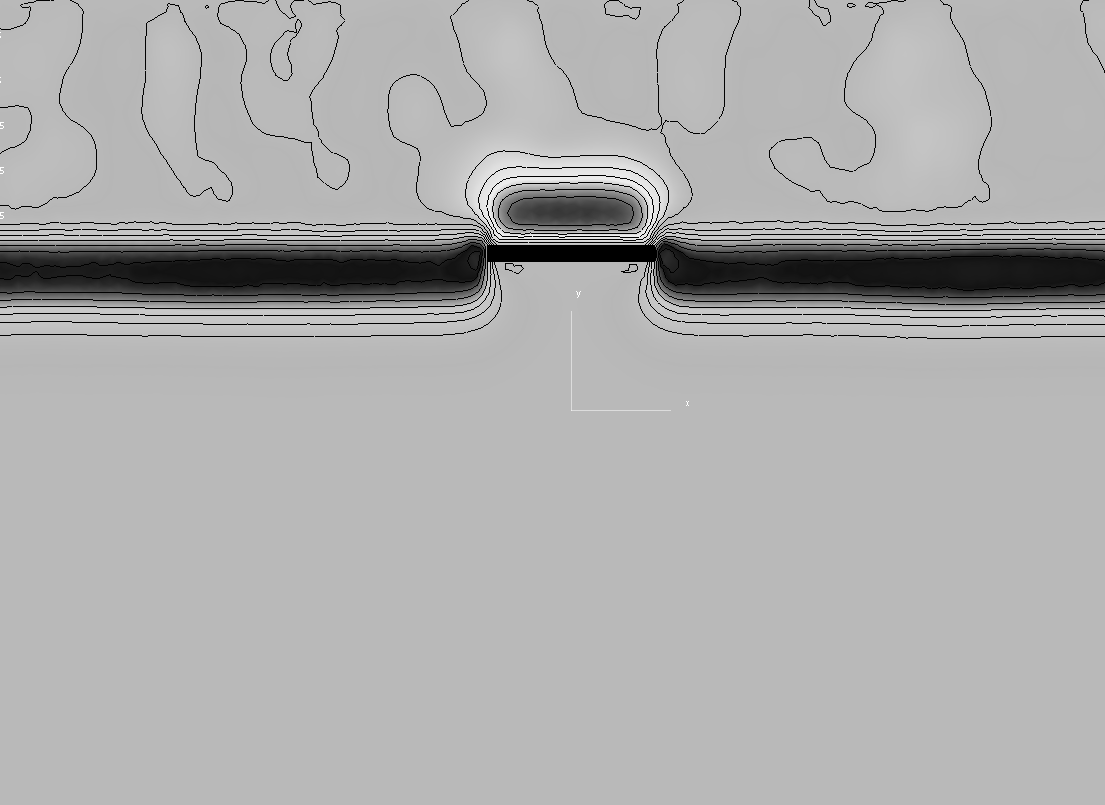
\includegraphics[width=\textwidth]{png/wave-around-crack/reflection-uniform-mesh.png}
\caption{Однородная мелкая сетка.}
\end{subfigure}
\begin{subfigure}[b]{0.5\textwidth}
\centering
\includegraphics[width=\textwidth]{png/wave-around-crack/reflection-non-uniform-mesh.png}
\caption{Сетки разной мелкости.}
\end{subfigure}
\caption{Начальный этап отражения волны нагрузки от раздробленной области. Напряжения в окружающем материале.}
\label{pic:crack_reflection}
\end{figure}

На рис. \ref{pic:crack_final_front} показан завершающий этап прохождения волнового фронта через раздробленную область. Форма фронта уже практически восстановилась после обтекания неоднородности. Видно, что при использовании неоднородной сетки интенсивность волны, отраженной от раздробленной области, несколько ниже. Уменьшение интенсивности прошедшего фронта, соответственно, тоже выражено менее явно. Тем не менее, на качественном уровне картина совпадает в обоих расчётах, нефизичных эффектов от использования неоднородных сеток не наблюдается.

\begin{figure}[htp]
\begin{subfigure}[b]{0.5\textwidth}
\centering
\includegraphics[width=\textwidth]{png/wave-around-crack/final-front-uniform-mesh.png}
\caption{Однородная мелкая сетка.}
\end{subfigure}
\begin{subfigure}[b]{0.5\textwidth}
\centering
\includegraphics[width=\textwidth]{png/wave-around-crack/final-front-non-uniform-mesh.png}
\caption{Сетки разной мелкости.}
\end{subfigure}
\caption{Отражённая волна и восстановление фронта проходящей волны за раздробленной областью.}
\label{pic:crack_final_front}
\end{figure}

